%%%%%%%%%%%%%%%%%%%%%%%%%%%%%%%%%%%%%%%%%%%%%%%%%%%%%%%%%%%%%%%%%%%%%%%%%%%%%
%%% LaTeX-Rahmen fuer das Erstellen von Bachelorarbeiten
%%%%%%%%%%%%%%%%%%%%%%%%%%%%%%%%%%%%%%%%%%%%%%%%%%%%%%%%%%%%%%%%%%%%%%%%%%%%%

%%%%%%%%%%%%%%%%%%%%%%%%%%%%%%%%%%%%%%%%%%%%%%%%%%%%%%%%%%%%%%%%%%%%%%%%%%%%%
%%% allgemeine Einstellungen
%%%%%%%%%%%%%%%%%%%%%%%%%%%%%%%%%%%%%%%%%%%%%%%%%%%%%%%%%%%%%%%%%%%%%%%%%%%%%

\documentclass[twoside,10pt,a4paper]{report}
\usepackage[utf8]{inputenc}
\usepackage[T1]{fontenc}

\usepackage{graphics, graphicx}
\usepackage{latexsym}
\usepackage[margin=10pt,font=small,labelfont=bf]{caption}



\usepackage[section]{placeins}
\usepackage{multirow}
\usepackage[table]{xcolor}
\usepackage{bussproofs}
\usepackage{tabu}
\usepackage{csquotes}
\usepackage{amsmath}
\usepackage{subcaption}
\usepackage{geometry}
\usepackage{mathpartir}
\usepackage{listings}
\usepackage{mathtools}
\usepackage{amssymb}
\usepackage{tikz}
\usetikzlibrary{positioning, calc, arrows, tikzmark}
\usetikzlibrary{shapes.multipart}
\usepackage{xcolor}
\definecolor{red}{HTML}{8c0000}
\definecolor{green}{HTML}{38775a}
\definecolor{blue}{HTML}{4054d6}
\usepackage{hyperref}
\usepackage{wrapfig}
\hypersetup{
    colorlinks,
    citecolor=black,
    filecolor=black,
    linkcolor=black,
    urlcolor=black
}
\usepackage{listings}
\lstset{
    mathescape=true,
    escapechar=|,
    language=SQL,
    showspaces=false,
    basicstyle=\footnotesize\ttfamily,
    extendedchars=true
}
\newcommand{\udfArg}[1]{{\$#1}}
\usepackage{minted}
\usemintedstyle{borland}
\newmintedfile[sqlcode]{postgresql}{
    fontfamily=tt,
    fontsize=\footnotesize,
    %linenos=true,
    %numberblanklines=true,
    %numbersep=5pt,
    %gobble=0,
    %frame=leftline,
    framerule=0.4pt,
    framesep=2mm,
    tabsize=2,
    obeytabs=false,
    mathescape=true,
    escapeinside=||,
    samepage=false, %with this setting you can force the list to appear on the same page
    showspaces=false,
    showtabs =false,
    texcl=false,
}
\setminted[postgresql]{fontsize=\footnotesize}

\newcommand*\circled[1]{\tikz[baseline=(char.base)]{
            \node[shape=circle,draw,inner sep=1pt] (char) {\tiny{\textbf{#1}}};}}
            
            
\newcommand{\markForTikz}[2]{\tikz[overlay,remember picture,baseline] 
\node [anchor=base] (#1) {$#2$};}

\newcommand{\DrawVLine}[3][]{%
  \begin{tikzpicture}[overlay,remember picture]
    \draw[shorten <=0.3ex, #1] (#2.north) -- (#3.south);
  \end{tikzpicture}
}

\newcommand{\DrawHLine}[3][]{%
  \begin{tikzpicture}[overlay,remember picture]
    \draw[shorten <=0.2em, #1] (#2.west) -- (#3.east);
  \end{tikzpicture}
}

% Do not make minted full width but only so wide as required
\RecustomVerbatimEnvironment{Verbatim}{BVerbatim}{}
\renewcommand{\figurename}{Listing}

\DeclareMathOperator{\FV}{\text{\rm FV}} % set of free variables
\DeclareMathOperator{\refs}{\ensuremath{\text{refs}}}
\DeclareMathOperator{\hasCallsite}{\ensuremath{\text{hasCallsite}_{fn}}}

\newcommand{\WITH}{\ensuremath{\text{\texttt{WITH}}}}
\newcommand{\AS}{\ensuremath{\text{\texttt{ AS }}}}
\newcommand{\SELECT}{\ensuremath{\text{\texttt{SELECT}}}}
\newcommand{\WHERE}{\ensuremath{\text{\texttt{WHERE}}}}
\newcommand{\FROM}{\ensuremath{\text{\texttt{FROM}}}}
\newcommand{\CASE}{\ensuremath{\text{\texttt{CASE}}}}
\newcommand{\WHEN}{\ensuremath{\text{\texttt{WHEN}}}}
\newcommand{\THEN}{\ensuremath{\text{\texttt{THEN}}}}
\newcommand{\ELSE}{\ensuremath{\text{\texttt{ELSE}}}}
\newcommand{\END}{\ensuremath{\text{\texttt{END}}}}
\newcommand{\AND}{\ensuremath{\text{\texttt{AND}}}}
\newcommand{\NOT}{\ensuremath{\text{\texttt{NOT}}}}
\newcommand{\TRUE}{\ensuremath{\text{\texttt{TRUE}}}}

\newcommand{\RREC}{\ensuremath{\text{\textsc{REC}}}}
\newcommand{\RREF}{\ensuremath{\text{\textsc{BASE}}}}
\newcommand{\RBASE}{\ensuremath{\text{\textsc{BASE}}}}
\newcommand{\REXPR}{\ensuremath{\text{\textsc{EXPR}}}}
\newcommand{\RWHEN}{\ensuremath{\text{\textsc{WHEN}}}}
\newcommand{\RELSE}{\ensuremath{\text{\textsc{ELSE}}}}
\newcommand{\RCTE}{\ensuremath{\text{\textsc{CTE}}}}
\newcommand{\RWITH}{\ensuremath{\text{\textsc{WITH}}}}
\newcommand{\RSELECT}{\ensuremath{\text{\textsc{SELECT}}}}
\newcommand{\RFROM}{\ensuremath{\text{\textsc{FROM}}}}
\newcommand{\RWHERE}{\ensuremath{\text{\textsc{WHERE}}}}

\setcounter{tocdepth}{4}
\setcounter{secnumdepth}{4}
%\textwidth 16cm
%\textheight 22cm
%\topmargin 0.0cm
%\evensidemargin 1cm
%\oddsidemargin 1cm
%\footskip 2cm
%\parskip0.5explus0.1exminus0.1ex

\providecommand*{\listingautorefname}{Listing}

\pagestyle{headings}

\sloppy
\begin{document}


% \highlight[<colour>]{<stuff>}
\newcommand{\highlight}[2][yellow]{\mathchoice%
  {\colorbox{#1}{$\displaystyle#2$}}%
  {\colorbox{#1}{$\textstyle#2$}}%
  {\colorbox{#1}{$\scriptstyle#2$}}%
  {\colorbox{#1}{$\scriptscriptstyle#2$}}}%

\newcolumntype{L}{>{$}l<{$}} % math-mode version of "l" column type

%%%%%%%%%%%%%%%%%%%%%%%%%%%%%%%%%%%%%%%%%%%%%%%%%%%%%%%%%%%%%%%%%%%%%%%%%%%%
%%% hier steht die neue Titelseite 
%%%%%%%%%%%%%%%%%%%%%%%%%%%%%%%%%%%%%%%%%%%%%%%%%%%%%%%%%%%%%%%%%%%%%%%%%%%%
 
\begin{titlepage}
 \begin{center}
  {\LARGE Eberhard Karls Universität Tübingen}\\
  {\large Mathematisch-Naturwissenschaftliche Fakultät \\
Wilhelm-Schickard-Institut für Informatik\\[4cm]}
  {\huge Master's Thesis Computer Science\\[2cm]}
  {\Large\bf Translating Recursive Functions to Declarative PostgreSQL User-Defined Functions\\[1.5cm]}
 {\large Stephan Biastoch}\\[0.5cm]
2018\\[4cm]
{\small\bf Reviewers}\\[0.5cm]
  \parbox{7cm}{\begin{center}{\large Prof. Dr. Grust}\\
  {\footnotesize Database Systems Research Group\\ Wilhelm-Schickard-Institut für Informatik\\%
	Universität Tübingen}\end{center}}\hfill\parbox{7cm}{\begin{center}
  {\large Prof. Dr. Klaus Ostermann}\\
  {\footnotesize Programming Languages \& Software Technology \\ Wilhelm-Schickard-Institut für Informatik\\%
	Universität Tübingen}\end{center}
 }
	
	%\begin{center}
%{\small\bf Betreuer}\\[0.5cm]
%{\large Name Betreuer}\\
%  {\footnotesize Adresse\\
%	Universit"at T"ubingen}\end{center}

  \end{center}
\end{titlepage}


%%%%%%%%%%%%%%%%%%%%%%%%%%%%%%%%%%%%%%%%%%%%%%%%%%%%%%%%%%%%%%%%%%%%%%%%%%%%
%%% Titelr"uckseite: Bibliographische Angaben
%%%%%%%%%%%%%%%%%%%%%%%%%%%%%%%%%%%%%%%%%%%%%%%%%%%%%%%%%%%%%%%%%%%%%%%%%%%%

\thispagestyle{empty}
\vspace*{\fill}
\begin{minipage}{11.2cm}
\textbf{Biastoch, Stephan:}\\
\emph{Translating Recursive Functions to Declarative PostgreSQL User-Defined Functions}\\ Master's Thesis Computer Science\\
Eberhard Karls Universit"at T"ubingen\\
Thesis period: 01.07.2018 - 31.12.2018
\end{minipage}
\newpage

%%%%%%%%%%%%%%%%%%%%%%%%%%%%%%%%%%%%%%%%%%%%%%%%%%%%%%%%%%%%%%%%%%%%%%%%%%%%

\pagenumbering{roman}
\setcounter{page}{1}

%%%%%%%%%%%%%%%%%%%%%%%%%%%%%%%%%%%%%%%%%%%%%%%%%%%%%%%%%%%%%%%%%%%%%%%%%%%%
%%% Seite I: Zusammenfassug, Danksagung
%%%%%%%%%%%%%%%%%%%%%%%%%%%%%%%%%%%%%%%%%%%%%%%%%%%%%%%%%%%%%%%%%%%%%%%%%%%%


%\newpage
\section*{Abstract}
%%%%%%%%%%%%%%%%%%%%%%
% Was ist das Thema? Welche Methoden? % Warum relevant? Wie Evaluiert? Was für Ergebnisse/Schlüsse?
%%%%%%%%%%%%%%%%%%%%%%
Relational database systems are a powerful way of working with vast amounts of complex data. Most industries rely on big data for everyday businesses, not to mention the recent ascend of machine learning. Usually, data is stored in databases and transferred into applications to perform complex computations. By leaving the database-world, we sacrifice everything that makes databases fast: Query planer, indices, optimized I/O and more. Furthermore, we have to take the overhead of retrieving the raw-data from the database-system.

Many complex and interesting computations on big data share a common property that makes most programmers switch instantly from SQL to any other programming language: Recursion. Writing recursive algorithms as recursive queries can be very challenging since most algorithms are designed in a functional or imperative style rather than data-oriented. User Defined Functions (UDFs) were introduced to ease development of complex queries and can even handle recursion -- but recursive UDFs are incredibly slow.

With our approach we give the programmer a fully automated tool that can be used to translate a recursive function, given by an SQL-UDF that is easy to write and maintain, into a single semantically equivalent query. The translation utilizes automatic memoization and removes the overhead from recursive UDFs. A first evaluation shows its efficiency for memoizable as well as divide-and-conquere algorithms. 

This thesis provides an operational semantics to analyze a given UDF statically and extract features required to construct the translation from a set of templates. This thesis is accompanied by a first implementation in Haskell for PostgreSQL.

%\input{0.2_Danksagung}
\newpage

%%%%%%%%%%%%%%%%%%%%%%%%%%%%%%%%%%%%%%%%%%%%%%%%%%%%%%%%%%%%%%%%%%%%%%%%%%%%%
%%% Inhaltsverzeichnis
%%%%%%%%%%%%%%%%%%%%%%%%%%%%%%%%%%%%%%%%%%%%%%%%%%%%%%%%%%%%%%%%%%%%%%%%%%%%%

\renewcommand{\baselinestretch}{1.3}
\small\normalsize

\tableofcontents

\renewcommand{\baselinestretch}{1}
\small\normalsize

\cleardoublepage

%%%%%%%%%%%%%%%%%%%%%%%%%%%%%%%%%%%%%%%%%%%%%%%%%%%%%%%%%%%%%%%%%%%%%%%%%%%%%
%%% Abbildungsverzeichnis
%%%%%%%%%%%%%%%%%%%%%%%%%%%%%%%%%%%%%%%%%%%%%%%%%%%%%%%%%%%%%%%%%%%%%%%%%%%%%

%\renewcommand{\baselinestretch}{1.3}
%\small\normalsize

%\addcontentsline{toc}{chapter}{Abbildungsverzeichnis}
%\listoffigures

%\renewcommand{\baselinestretch}{1}
%\small\normalsize

%\cleardoublepage

%%%%%%%%%%%%%%%%%%%%%%%%%%%%%%%%%%%%%%%%%%%%%%%%%%%%%%%%%%%%%%%%%%%%%%%%%%%%%
%%% Tabellenverzeichnis
%%%%%%%%%%%%%%%%%%%%%%%%%%%%%%%%%%%%%%%%%%%%%%%%%%%%%%%%%%%%%%%%%%%%%%%%%%%%%

%\renewcommand{\baselinestretch}{1.3}
%\small\normalsize

%\addcontentsline{toc}{chapter}{Tabellenverzeichnis}
%\listoftables

%\renewcommand{\baselinestretch}{1}
%\small\normalsize

%\cleardoublepage

%%%%%%%%%%%%%%%%%%%%%%%%%%%%%%%%%%%%%%%%%%%%%%%%%%%%%%%%%%%%%%%%%%%%%%%%%%%%%
%%% Abk"urzungsverzeichnis
%%%%%%%%%%%%%%%%%%%%%%%%%%%%%%%%%%%%%%%%%%%%%%%%%%%%%%%%%%%%%%%%%%%%%%%%%%%%%

%\addcontentsline{toc}{chapter}{Abk\"urzungsverzeichnis}
%\input{0.3_Abkuerzungen}

%\cleardoublepage

%%%%%%%%%%%%%%%%%%%%%%%%%%%%%%%%%%%%%%%%%%%%%%%%%%%%%%%%%%%%%%%%%%%%%%%%%%%%%
%%% Der Haupttext, ab hier mit arabischer Numerierung
%%% Mit \input{dateiname} werden die Datei `dateiname' eingebunden
%%%%%%%%%%%%%%%%%%%%%%%%%%%%%%%%%%%%%%%%%%%%%%%%%%%%%%%%%%%%%%%%%%%%%%%%%%%%%

\pagenumbering{arabic}
\setcounter{page}{1}

%% Introduction
\chapter{Introduction}\label{Introduction}
%%%%%%%%%%%%%%%%%%%%%%
% Was wurde untersucht? Was ist daran neu?
% Warum ist das schwierig? Was sind die Herausforderungen?
% Warum relevant?
% Was leistet meine Arbeit? Welche wiss. Beiträge leiste ich?
% Was gibt es für ähnliche Arbeiten? Wie ist meine Anders?
% Der Fahrplan: Wie ist die Arbeit aufgebaut?
%%%%%%%%%%%%%%%%%%%%%%

%    What is the problem?
%    Why is it interesting and important?

\paragraph*{Motivation} Recursion is concise and easy to understand and write, since it resembles our inductive way of thinking about recursive tasks. We start from a nonrecursive basecase and then construct the recursive cases. Evaluation happens by stacking up recursive calls until basecases are reached and first result can be assemble from them.

The problem with recursion in general is that it comes with a large overhead. Each call that waits on the result of other function calls is "paused" and the state of execution is pushed to the callstack. This is very expensive in terms of time and memory. All variables, returning addresses etc. need to be copied to the stack when switching the context, and restored when popping the layer. For SQL-UDFs, each call comes with especially large overhead because the UDF-body of every function is planned and the plan needs to be saved until the call returns. Therefore, recursive procedures in SQL are very slow and the limited stack size is quickly exceeded.

%    Why is it hard? (E.g., why do naive approaches fail?)
Iterative solutions with dynamic programming are usually the way to go where recursion is impractical. By iteratively manipulating variables inside the heap memory, much overhead from the recursion can be avoided. Additionally, computation is not restricted by stack depth (megabytes) but by heap sizes (gigbytes). Dynamic Programming aims to avoid redundant recursive calls by saving results of subproblems in a table. Translating a declarative but inefficient algorithm into an imperative language like Java and implementing dynamic programming can be challenging. If you can exploit specific mathematical properties of the problem to constraint the search space, you may come up with a very efficient solution. But this is a time consuming task and developer time is always a very limited resource.

If your target language is not an imperative language but a declarative SQL-query, implementation is less straight forward. You will additionally need a decent amount of knowledge of SQL, the query planner and probably other internals of the database system to avoid all the pitfalls that can slow down your query. Additionally, you sacrifice much readability for performance, obfuscating the logical level with implementation details. This makes the query less maintainable and more error prone.

%    Why hasn't it been solved before? (Or, what's wrong with previous proposed solutions? How does mine differ?)
Our approach fully automatizes the optimization process so that the programmer can keep maintaining a truly declarative UDF in a functional style without concerns of performance. The recursive UDF is automatically translated into an optimized formulation implementing Memoization. The translation is based on slicing the original function into its different evaluation scenarios. The callsite-arguments of the current scenario are evaluated independently from the surrounding context, creating the callgraph. The callgraph is then level-wise evaluated.

\paragraph*{Example}

% fib example
As example, let us comprehend how the Fibonacci function is translated. It is defined as $F_n = F_{n-1} + F_{n-2}$ with $F_0 = 0$ and $F_1 = 1$ \cite[p. 79]{TAOCP_Knuth}. For this example we will use the (slightly awkward) formulation from figure \autoref{intro_fib}. We require that all case-distinctions in the query are made by an explicit \texttt{CASE}-expression.

\begin{figure}[h]\small
    \begin{minipage}[b]{.47\linewidth}
        \input{tikz/fib_callstack.tex}
        \caption{Callstack-growth of \texttt{fib(4)}}
        \label{fib_4_callstack}
    \end{minipage}\hfill
    \begin{minipage}[b]{.5\linewidth}
    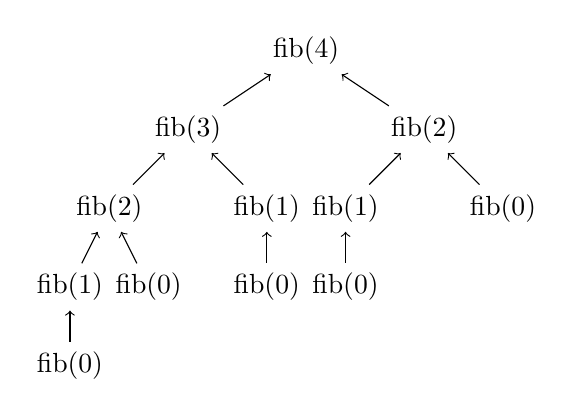
\begin{tikzpicture}
% nodes
\node (n1)     at (2.5, 2) {fib(4)};
    \node (n1-1)   at (1, 1) {fib(3)};
        \node (n1-1-1) at (0, 0) {fib(2)};
            \node (n1-1-1-1) at (-0.5, -1) {fib(1)};
                \node (n1-1-1-1-0) at (-0.5, -2) {fib(0)};
            \node (n1-1-1-2) at (0.5, -1) {fib(0)};
        \node (n1-1-2) at (2, 0) {fib(1)};
            \node (n1-1-2-0) at (2, -1) {fib(0)};
    \node (n1-2)   at (4, 1) {fib(2)};
        \node (n1-2-1) at (3, 0) {fib(1)};
            \node (n1-2-1-0) at (3, -1) {fib(0)};
        \node (n1-2-2) at (5, 0) {fib(0)};
% arrows
\draw[<-] (n1)     -- (n1-1);
\draw[<-] (n1)     -- (n1-2);
\draw[<-] (n1-1)   -- (n1-1-1);
\draw[<-] (n1-1)   -- (n1-1-2);
\draw[<-] (n1-2)   -- (n1-2-1);
\draw[<-] (n1-2)   -- (n1-2-2);
\draw[<-] (n1-1-1) -- (n1-1-1-1);
\draw[<-] (n1-1-1) -- (n1-1-1-2);
\draw[<-] (n1-1-1-1) -- (n1-1-1-1-0);
\draw[<-] (n1-1-2) -- (n1-1-2-0);
\draw[<-] (n1-2-1) -- (n1-2-1-0);
\end{tikzpicture}
        \caption{Callstack-evaluation of \texttt{fib(4)}}
        \label{fib_4_callstack_evaluation}
    \end{minipage}
\end{figure}

% Recursive evaluation in SQL
What happens if we call \mintinline{postgresql}{SELECT fib(4)}? The planner takes some time to have a close look at the query inside fib to make an execution plan and then executes this plan. During execution, a number of subcalls occurs that need to be executed before the surrounding query can be evaluated. Everytime, the UDF is replanned and a callstack will grow as illustrated in \autoref{fib_4_callstack}. As soon as a node has the result of all of its children, the node can itself return a result. The leaves of the tree can therefore return a result immediately and the evaluation starts bottom-up (\autoref{fib_4_callstack_evaluation}). 


\begin{figure}[h!]
    \begin{minipage}[b]{.45\linewidth}
    \centering\large
    \sqlcode{snippets/fib_wide.sql}
    \vspace{8mm}
    \subcaption{SQL UDF returning the nth Fibonacci number}
    \label{intro_fib}
    \end{minipage}\hfill
    \begin{minipage}[b]{.45\linewidth}
    \centering\small
    \vspace{-8mm}
    
    \begin{align*}
\Big(&\big\{&\big\langle~&\text{pred}:     &\mintinline{postgresql}{SELECT ($1 = 0)}                  &\\
    &      &    ,~      &\text{query}:    &\mintinline{postgresql}{SELECT 0}                          & \big\rangle \big\}\\
, ~ &\big\{&\big\langle~&\text{pred}:     &\mintinline{postgresql}{SELECT (NOT $1 = 0) AND ($1 = 1)}&\\
    &      &    ,~      &\text{query}:    &\mintinline{postgresql}{SELECT 1 + fib(0)}&    \\
    &      &    ,~      &\text{callsites}:&\langle \text{id}: 1,~\text{args}: (\mintinline{postgresql}{SELECT 0})\big\rangle & \big\rangle\\
    &      &\big\langle~&\text{pred}:     &\mintinline{postgresql}{SELECT (NOT $1 = 0) AND (NOT $1 = 1)}&\\
    &      &    ,~      &\text{query}:    &\mintinline{postgresql}{SELECT fib($1 - 1) + fib($1 - 2)}&\\
    &      &    ,~      &\text{callsites}:&\langle \text{id}: 2,~\text{args}: (\mintinline{postgresql}{SELECT $1 - 1})\rangle &,\\
    &      &            &                 &\langle \text{id}: 3,~\text{args}: (\mintinline{postgresql}{SELECT $1 - 2})\rangle & \big\rangle\big\} \Big)
    \end{align*}
    \subcaption{Recursive scenarios}\label{fib_rec_scenarios}
    \end{minipage}
    \caption{Output of scenario analysis of \mintinline{postgresql}{fib(int)} from \autoref{intro_fib}}\label{fib_analysis_output}
\end{figure}


\begin{wrapfigure}{r}{0.4\linewidth}
\centering
\begin{tabular}{@{}|c|c|c|@{}}
  \tabname{2}{\strut\texttt{\,callgraph\,}} \\
  \colhd{in\_1} & \colhd{callsite\_id} & \colhd{out\_in} \\
  4 &  2 & 3 \\
  4 &  3 & 2 \\\hline
  3 &  2 & 2 \\
  3 &  3 & 1 \\
  2 &  2 & 1 \\
  2 &  3 & 0 \\\hline
  1 &  1 & 0 \\
  \hline
\end{tabular}
\caption{}\label{tbl:callgraph}
\end{wrapfigure}

% Callgraph creation
The idea behind the translation is to simulate this two phases: top-down callstack-growth and bottom-up evaluation. The callstack is created by evaluating only the parts of the UDF that are necessary to observe subsequent recursive calls. First, this are the predicates of the \texttt{CASE}-expression. They are required to detect which callsites are actually called with the given UDF-arguments. Second, the arguments of these callsites need to be evaluated to find out the input-arguments for the subsequent calls. This way, the callstack is built until all callsites lead to basecases. By collecting only unique rows, it is actually not a callstack but a \textit{callgraph} that we create as it contains no duplicate calls.



%To generate the callstack we need to keep track of subsequent calls. To achieve this, we slice the UDF into all possible evaluation scenarios together with predicates to test if a scenario is executed with the current arguments. Now, we can evaluate the \textit{arguments} of the callsites of the current scenario and add subseqent calls to the callstack by this. Substituting the original call arguments (eg. \texttt{\$1} or \texttt{n}) with a reference to the newly discovered arguments from the previous iteration, we are able to generate a complete callstack.

\begin{wrapfigure}{l}{0.35\linewidth}
\centering
\begin{tabular}{@{}|c|c|@{}}
  \tabname{2}{\strut\texttt{\,evaluation\,}} \\
  \colhd{in\_1} & \colhd{result} \\
  \texttt{0} & \texttt{0} \\\hline
  \texttt{1} & \texttt{1} \\\hline
  \texttt{2} & \texttt{1} \\\hline
  \texttt{3} & \texttt{2} \\\hline
  \texttt{4} & \texttt{3} \\\hline
\end{tabular}
\caption{}\label{tbl:evaluation}
\end{wrapfigure}

% Callgraph evaluation
Evaluation starts from the bottom: The leaves of the the callstack, ie. the basecases, do not contain any callsites and can therefore evaluated directly and saved. From here evaluation ascends the callstack again and callsites are replaced with references to their results. As soon as all callsites of a scenario have results available, the scenario can be evaluated. This continues until the entire callstack is evaluated and the final result can be returned.


%The idea of the callstack CTE is to collect in every step the arguments of the newly occuring recursive calls. With the data of the analysis, this is a simple task. The following pseudocode gives you an intuition: \mintinline{postgresql}{SELECT in_args, callsite.id, callsite.args FROM scenario.pred p WHERE p.v}. This snippet returns the arguments of a callsite within a scenario that is called with the given \texttt{in\_args} if the predicate of the scenario evaluates to true. If we do this for every callsite in every scenario, we receive a complete level in the tree of the callstack (see \autoref{discovery_strucutre}). To compute the complete callstack, we need to iterate over every set of arguments from the previous call (ie. the level above) and continue collecting calls until no new calls are outputed since we reached the basecases. See \autoref{callstack_recurse} for an illustration.

%By collecting all calls in a table it is also trivial to remove duplicate calls from the callstack before evaluation (figure z), which gives us memoization which speeds up the translation significantly. The callstack table is just a relational representation of the callstack with memoization (Table T).

The output function is generated by filling out a query-template. The data to be filled in is an intermediate representation of the input UDF (\autoref{}), which is generated by a syntax driven analysis of the UDF (\autoref{chapter:analysis}). Its main part is the \textit{scenario analysis} which "slices" the UDF into its different evaluation scenarios. Each scenario consists of a predicate and a query that is semantically equivalent to the original function if the predicate is fulfilled. From the different scenarios the intermediate representation is created. Additional, special properties of the UDF (eg. tail recursion) are detected to choose the best template.

\iffalse
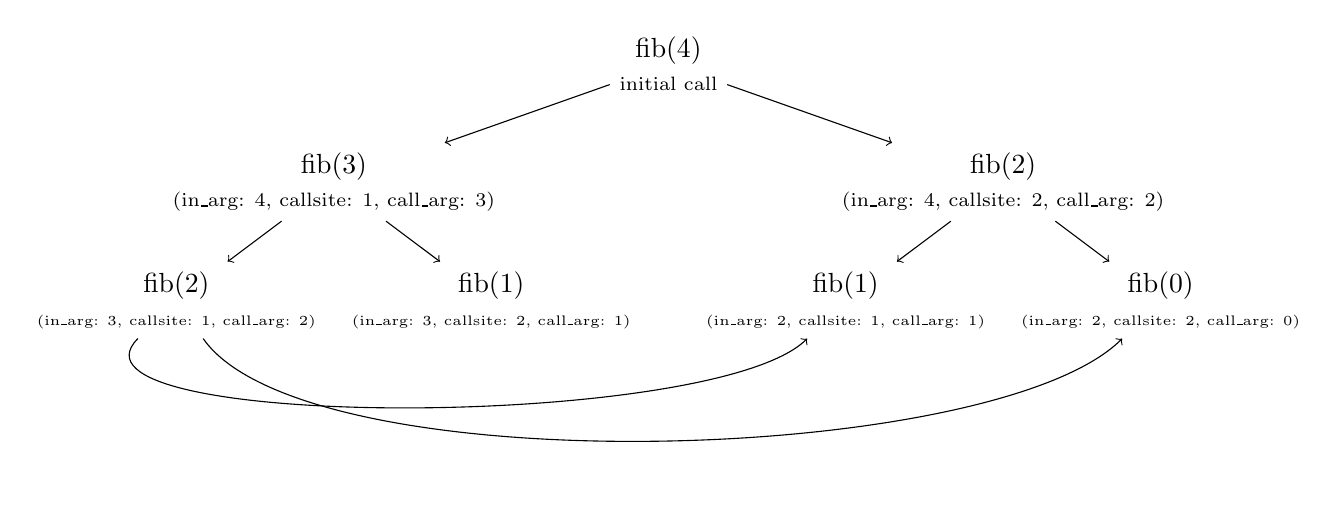
\begin{tikzpicture}[->, level distance=15mm, align=center]
\tikzstyle{level 1}=[sibling distance=85mm]
\tikzstyle{level 2}=[sibling distance=40mm]
\tikzstyle{level 3}=[sibling distance=40mm]
\node{fib(4)\\\scriptsize{initial call}}
  child { node {fib(3)\\\scriptsize{(in\_arg: 4, callsite: 1, call\_arg: 3)}}
    child {node (fib2) {fib(2)\\\tiny{(in\_arg: 3, callsite: 1, call\_arg: 2)}}
      %child {node {fib(1)\\\tiny{(in\_arg: 4, callsite: 2, call\_arg: 2)}} }
      %child {node {fib(0)\\\tiny{(in\_arg: 4, callsite: 2, call\_arg: 2)}} }
    }
    child {node (fib1) {fib(1)\\\tiny{(in\_arg: 3, callsite: 2, call\_arg: 1)}} }
  }
  child {node {fib(2)\\\scriptsize{(in\_arg: 4, callsite: 2, call\_arg: 2)}}
    child {node (fib1) {fib(1)\\\tiny{(in\_arg: 2, callsite: 1, call\_arg: 1)}} }
    child {node (fib0) {fib(0)\\\tiny{(in\_arg: 2, callsite: 2, call\_arg: 0)}} }
  };
\draw[->, bend left=10, out=225, in=225, looseness=0.5] (fib2) edge (fib1);
\draw[->, bend right=5, out=305, in=225, looseness=0.5] (fib2) edge (fib0);
\end{tikzpicture}
\fi

%Based on the recursive scenarios, all callsites are enumerated and their arguments extracted to self-contained queries. The recursive cases are enriched with a list of callsites they contain to check later on whether a result for all callsites of an recursive scenario is present yet.
% Callsite 1: (Argument 1: SELECT \$1 - 1); Callsite 2: (Argument 1: SELECT \$1 - 2)
  
%Now we have all the data required to construct a query that assembles the callgraph. This is achieved by recursivly collecting the arguments of the callsites of those scenarios that occur under the given input argeters. In the beginning, the original input argeters of the function are used. As we recurse, we iterate through the newly added callsite arguments to collect data of further calls. We end up by a relational encoding of a callgraph.

%\sqlcode{snippets/fib_discovery.sql}

%, tracking calls down to the basecases (ie. the nonrecursive scenarios) without evaluating anything from the original function except the callsite-arguments. After the creation of the callgraph, we know the input argeters for the basecases and can evaluate them. With the results of the basecases at hand, it is now possible to continue evaluation up the callgraph. For each recursive scenario we check if for all contained callsites with the given input arguments, a result already exists. If so, the call in the recursive scenario is replaced with the reference to the result and the recursive scenario can be evaluated.

% What are the key components of my approach and results? Also include any specific limitations. 
%The translation of an UDF is split in two major parts, static analysis and template expansion. During static analysis the original UDF is split into different evaluation scenarios with a predicate under that this scenario will be evaluated. The analysis result is used to choose and fill appropriate templates to build the translated function.

%\paragraph*{Static analysis}
%Case analysis: 
%Callsite extraction
%Recursion type detection
%Constant argeter detection
%Hashability checks

%This thesis goal is to extend to range of algorithms for which it is easy to write a fairly performing implementation in standard SQL. I provide inference rules to perform a syntax directed analysis of a given SQL UDF that extracts evaluation scenarios alongside with conditions under which each scenario is executed. To analyze the query correclty, it is necessary to track direct and indirect references to callsites while analyzing the query. Callsites are tracked through FROM, subqueries and CTEs and also takes shadowing into account. Extracted scenarios also contain only actually referenced CTEs, deleting unused CTEs that were referenced by other WHEN-branches. The extracted predicates do not contain any callsites so that they can be used to guard the execution of the scenarios. Predicates, Scenarios and Callsite arguments are extracted in a closed form, so that they contain no free variables and can be evaluated independenty from each other. To achieve this, none of these may reference a row-variables from an outside FROM, only table-variables may be referenced, including outside CTEs. This also limits the ability of the UDF to perform meaningful computations that return tabular results, which we forbid entirely for now.

%Each scenario is generated from the different branches of a \CASE-statement and the predicates that need to be fulfilled to reach a given \WHEN-branch. Each resulting scenario is semantically equivalent to the original query if its predicate is fulfilled. All scenarios combined are semantically equivalent to the original query. The scenarios are divided into basecases, that do not contain any recursive callsites, and recursive cases that do contain one or more callsites. Some more analysis is performed on the generated scenarios to detect properties of the function like tail recursion.



%\paragraph*{Template-based translation}
%Callstack
%Basecases
%TerminationCheck
%Evaluation
% From the extracted data an appropriate template is filled, forming the translation. The translation utilizes the iterative nature of WITH RECURSIVE to implement an actual iterative version of the recursive UDF. First, the callstack is discovered by iterativly collecting the new arguments of the callsites in the appropiate scenario. Second, the basecases are evaluated and all new computable results are collected. This repeats until the final result is computed. Cases where the translation would terminate but the original does not are detected and an infinite loop is created to mimic the original behaviour.

% The translation template consists of a discovery-phase and an evaluation-phase. During discovery the callstack is built, collecting all recursive calls down to the nonrecursive basecases. From the discovery-table it is now possible to look up the input arguments that lead to a nonrecursive scenario which can be used to begin the recursive evaluation process. As soon as results for all callsites of a given scenario exist, this scenario can be evaluated. The query continues recursively until the argeter of the original call is found in the evaluation table.
    
\paragraph*{Contributions} The general translation idea has been developed at the Database Systems Research Group at WSI in Tübingen. My main contribution is a first working implementation of this approach in Haskell, targeting PostgreSQL 10.6. I provide a handy command line tool \texttt{twr} to perform translations of UDFs from the database or from a SQL-file. A folder of UDFs or even an entire database can be batch-translated. The translated function(s) can be renamed and saved to file/folder or persisted in the database. Optimizations can selectively be disabled and analysis output can be shown.

Beside a first working implementation, I contributed some improvements to the inference rules to slice the original UDF into its evaluation scenarios. Here, my main contribution is the addition of rules to handle CTEs that may be nested and can contain callsites. Further, I have rewritten the rules for handling case-expressions to work in a step-wise fashion. This allows recursive predicates that contains nested \texttt{CASE}-expressions. The step-wise operation also made implementation easier. I added also a set of simple rules to extract the arguments from callsite while keeping references to used CTEs.

I also contributed a number of improvements to the templates. Most notably, I have rewritten the template for evaluating recursive scenarios that removes array aggregation and thereby allows arbitrary array arguments\footnote{When aggregating arrays, \texttt{array\_agg} requires all arrays to have the same dimensionality. This renders non-constant array arguments impossible.}. Furthermore, I simplified result selection and non-termination by adding the original call to the callgraph. The pattern to stop evaluation of the recursive CTE when no new results are created while adding old results to the result was also created by me.

% There are two interesting parts regarding the translation. The first is the template itself and its various optimizations that can be applied under certain circumstances, eg. when the function is tail recursive. The other interesting part is how to derive the sliced representation of the UDF that is required to fill the templates. I provide a small-step operational semantics over a subset of SQL to compile a query into its scenarios.

% First I will establish the backgrounds required for this thesis. The evaluation of SQL-queries, which is important to understand query performance, is covered first. Special focus is laid on the evaluation of WITH RECURSIVE which we utilize to create a translation from a recursive to an actually iterative function. The evaluation of SQL-UDFs is covered then, showing differences in evaluation that lead to the poor performance of recursive UDFs. Important forms of recursion, as well as pros and cons are dicussed afterwards. The background-chapter closes with a short primer on Small step Operational Semantics.
\newpage

%%
\chapter{Background}\label{Introduction}

\section{Relational Databases}\label{theory}

In this chapter I give a short overview about aspects from the area of (relational) database systems that are relevant to my thesis. I introduce the relational data model and its Structured Query Language (SQL). All explanations target PostgreSQL 10.6 as state-of-the-art Database Management System (DBMS).

PostgreSQL 10.6 is used throughout this thesis as RDBMS and SQL-dialect. Its first version was developed as "POSTGRES" at Berkely 1986 \cite[xxxvi ff.]{psql}. It had its first open source release under the name "Postgres95" in 1995 where the own query language PostQUEL was replaced by SQL. As of 1997 and version 6.0 the software is named "PostgreSQL" to reflect its SQL-capabilities \cite[xxxvi ff.]{psql}.

PostgreSQL claims to be "the most advanced open-source database available anywhere" \cite[xxxvii]{psql}. It conforms to most parts of Core SQL:2011 \cite[S. 2198]{psql} and offers great extensibility and introspection. User defined functions, types, operators, index methods, statistics for the planner, procedural languages, foreign data wrappers and rewrite rules are possible. 

\subsection{Relational Data Model}
An integral part of many applications is to retrieve, modify and persist data. Depending on the complexity of the data (eg. plain key-value, hierarchical structured, associations to other data, etc.) and the requirements to the storage system (performance, query capabilities, robustness, multi-user capability, etc.) a number of solutions are viable. Relational Database Management Systems (RDBMS) are a very popular and advanced solution to manage vast amounts of interconnected data efficiently.

The original relational data model dates back to 1970 where E. F. Codd proposes a representation of data in set-theoretic \textit{relations} \cite{codd}. A relation is similar to \textit{table} with named and typed \textit{columns}. An instance of a relation is a set of tuples from the \textit{domain} of each of the columns. A subset of columns in a relation may form a unique \textit{primary key} for each of its tuples that can be included in other tables as \textit{foreign key} to establish references. A relational data model should be normalized to remove redundancies and enforce atomacity.

An important innovation by the relational model was the claim that access of the stored data should be separated from its internal (physical) representation and should be able to change without affecting the logical representation that is used by a program (\textit{data independence}). Instead of manually accessing the physical stored data, the programmer should just use a "data base sublanguage" (Codd) to specify tasks on the logical level, and the DBMS finds automatically an efficient way to perform the task on a physical level \cite[p. 3 ff.]{FoD}.

Based on Codds proposal of a "universal data sublanguage" to define and manipulate a relational model, Chamberlin and Boyce designed a "Structured English Query Language" (SEQUEL) \cite{sequel, sequel2}. The name alone highlights its declarative nature: Say \textit{what} you want, just in simple English. SEQUEL was later renamed to SQL and first standardized in 1987 as SQL:86 (ISO 9075:1987), the latest version to date is SQL:2016 (ISO/IEC 9075:2016). For this thesis, only a subset of the \textit{Data Manipulation Language} (DML) is of interest, namely reading queries.

\subsection{SQL and query evaluation}

Due to their declarative nature, SQL-Queries are no executable programs by themselves. To create an program from the query (a \textit{plan}), it is first parsed into an \textit{Abstract Syntax Tree} (AST, \autoref{fig:fib_ast}). An AST encodes the syntactic structure of the query into the structure of the AST, preserving its semantics. Parsing text into an AST is a standard step in compilation because ASTs are much more suitable to work with \cite[p. 5]{dragenbook}.

\begin{figure}[h!]
    \centering\footnotesize
    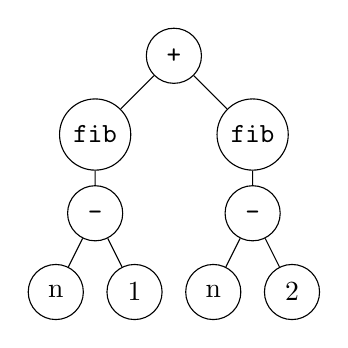
\begin{tikzpicture}[level distance=1cm,level 1/.style={sibling distance=2cm},level 2/.style={sibling distance=1cm}, every node/.style = {shape=circle, draw, align=center, minimum width=7mm, minimum height=7mm}]]
    \node {\texttt{+}}
        child { node{\texttt{fib}}
            child { node {\texttt{-}}
                child { node {n} }
                child { node {1} }
            }
        }
        child { node{\texttt{fib}}
            child { node {\texttt{-}}
                child { node {n} }
                child { node {2} }
            }
        };
    \end{tikzpicture}
    \caption{AST of \texttt{fib(n-1) + fib(n-2)}}
    \label{fig:fib_ast}
\end{figure}

The \textit{parse-tree} of the input query is transformed into a \textit{query-tree}. The transformation to the query-tree includes some desugering like expanding \texttt{T.*} to an explicit column-list, adding default \texttt{ELSE NULL} to \texttt{CASE}-statements and expanding row-comparisons \texttt{(1, 2) = (1, 4)} to boolean conjunctions \texttt{1=1 AND 1=4}. This makes it easier for the query planner to analyze the structure of the query and derive an efficient plan. Finally the query is rewritten, which primary replaces references to views by their original queries. \cite{}

The preprocessed and rewritten query is then fed into the \textit{query planner} to compile the declarative query into an procedural program (a \textit{plan-tree}) executable by the \textit{executor}. Its main responsibility is to find the fastest way to access and join the involved tables. Every (nontrivial) plan has table scans at its leafs. There are multiple ways to scan a table depending on the presence of predicates and auxiliary datastructures (\textit{indices}). Consider the query \texttt{SELECT * FROM T WHERE T.v = 5}. Depending on the size of \texttt{T} and the number of occurrences of \texttt{5} in the column \texttt{T.v} it may be most efficient to do a full \textit{sequential scan} of the entire table, filtering out rows not matching the predicate. If the table is large and there are only few rows with \texttt{T.v = 5}, an \textit{index-scan} may be much faster. With few I/O-operations the matching rows can be selectively retrieved, without reading the entire table. Various statistics are maintained to help the planner estimate the cost for each operation and choose the cheapest plan. \cite[p. 1887]{psql}


Tables in the \texttt{FROM}-clause can be combined (\textit{joined}) by different algorithms. Each algorithm has its own preconditions, strengths and weaknesses, so the choice of the appropriate join-strategy is very important. As each join-algorithm expects exactly two input tables, joining multiple tables results in a binary join-tree. The join order can impact the query performance dramatically as it determines the size of the intermediate join-results. Three tables R, S, T can either be joined as $(R \bowtie S) \bowtie T$ or as $R \bowtie (S \bowtie T)$. In general it is beneficial to choose the option that removes most rows from the result early to avoid investing time in joining rows that are eventually removed. The planner tries to attach predicates from the query to the joins to reduce the size of the join result (\textit{predicate push-down}).

Further nodes in the plan are used for sorting, aggregation, combining queries and others. Obviously, there are a lot of possible plans for a single query. To find the best plan, the query planner computes all possible plans and estimates the cost of each solution based on various statistics to select the cheapest. As the search-space for the planner growths exponentially with the number of involved tables, the exhaustive search switches to a heuristic-driven optimization when a threshold is exceeded \cite[p. 2064 ff.]{psql}.


Finally, the \textit{executor} recursively executes each node of the plan just as long as required by the parent node (Volcano Iterator Model) \cite{volcano}. Thus, each operation is not necessarily performed to completion but just as long as required to return the next row. Each plan contains therefore not only an estimate for the \textit{total cost} of the node until completion, but also minimum cost to return the first row (\textit{start up cost}). In the best case, the first returned row is just the single requested row and eg. the entire remaining table scan can be omitted. Yet, some operations need to be run to completion before being able returning the first row, eg. sorting. For these cases, the start up cost equals the actual cost.




% Building the cartesian product between tables is called a \textit{join}. Even for moderate sized tables the result of a couple of joins can be astronomically large, if done naively. Imagine build the cartesian product a table \texttt{S} with 10.000 rows, \texttt{T} with 100 rows and \texttt{R} with 1.000 rows. The resulting table would have $10.000 * 100 * 1.000 = 1.000.000.000$ rows - that escalated quickly!

% They just specify \textit{what} the user wants to achieve without telling \textit{how} (declarativity \cite[p. 21]{ullman}). To understand the "problem statement" of the user, the query is parsed, checked and rewritten before fed into the query-planner.

% It is possible to output the generated parse- and query-trees to the logfiles with configuration parameters \texttt{debug\_print\_\{parse, rewritten\}} set to true. To sanitize and parse the query-tree again, I used the great library \texttt{PgQueryHauler} by Denis Hirn \cite{denis_hirn} and Peter Richter \cite{peter_richter} to parse the logs and pretty print them as SQL again.

% There may be many possible strategies to execute a query and the best solution depends on various details (physical organization, frequencies of values, auxiliary data-structures, etc. pp) that may help to find the most efficient one. The \textit{query planner} is responsible to generate an actual executable, imperative program called a \textit{plan}.

%They specify \textit{what} the user wants to achieve without requiring any information about the exact \textit{how}. A query to count the number of rows with \texttt{t=0} from a table \textit{T} does state this intent directly as \texttt{SELECT COUNT(*) FROM T WHERE t = 0}. There is no loop incrementing a counter nor any information included about the location or retrieval of the contents of \texttt{T}. The desired result is specified at a high abstraction level and the best way to compute this result is obtained automatically. This property is known as \textit{declarativity}.

% To evaluate the query, the "problem statement" (the query) needs to be translated into a concrete "plan". This translation is done by the query planner.

% But even the query planner is not the holy grail and there are queries that perform incredibly bad or are difficult to formulate in a way the query planner can find a efficient plan.

% The most frequent form of reading queries are $\textit{SELECT s_1, s_2, ..., s_n FROM T_1, T_2, ..., T_n WHERE p}$-queries (S-F-W). The cartesian product $\texttt{T_1 \times T_2 \times \dots \times T_n}$ between the tables is built and the resulting rows are filtered by the predicate \texttt{p}. Finally, the output columns in the select-list are evaluated for each row, returning the output table.
\section{Recursion in SQL}

Recursion is a fundamental concept in everyday programming as well in computability-theory. Every recursive function consists of a number of different \textit{evaluation scenarios}. Some of them cause subsequent recursive calls (\textit{recursive scenarios}) and at least one scenario causes no recursive calls at all. Otherwise, the function will never terminate. We will call nonrecursive scenarios \textit{basecases}. The programmer usually uses conditionals to direct which scenario should be evaluated. For this thesis, I assume that conditionals are given in the form of \texttt{CASE}-expressions only, to that a \textit{predicate} is stated explicitly for each scenario. One of the main task of the translation is to collect the scenarios and identify their predicates.

Recursive functions can be implemented in SQL in two ways: As User Defined Function (UDF) or as self-referential Common Table Expression (CTE) in \texttt{WITH RECURSIVE}-queries. UDFs are functions (actually procedures) as we know them: A function with a name, an argument list, a defined return type and a function body. Recursive CTEs are different, as they are no procedures with explicit arguments but self-referential queries of a specific structure.

\subsection{Recursive User Defined Functions}
Recursive functions can be created in PostgreSQL as UDFs. UDFs can be implemented in a wide range of languages but we consider only SQL-UDFs as the pure SQL approach. There is also a number of ways to specify arguments and add modifiers. For my thesis I use just simple positional arguments without any modifiers (eg. \texttt{\$1}).

\begin{figure}[h!]
    \centering
    \begin{minted}{postgresql}
CREATE FUNCTION fac(INT) RETURNS INT AS $$
SELECT CASE WHEN $1 = 1 THEN 1
            ELSE $1 * fac($1 - 1)
       END
$$ LANGUAGE SQL;

SELECT fac(10);
    \end{minted}
    \caption{Calculation of $10!$ using a a recursive UDF \texttt{fac)}.}
    \label{fig:my_label}
\end{figure}

A UDF is mostly a black box for the query planner. They have just a fixed cost assigned as a whole (default 1000 \cite[p. 1435]{psql}) and the body of every call is repeatedly planned before execution.

Under certain circumstances, PostgreSQL can optimize some function calls. Very simple functions can be inlined during planning \cite{psqlWikiUDFinlining}  (see \autoref{fig:inlining}), but this is done only once, so its impact for recursive functions is not a game-changer.


\begin{figure}[h!]
    \centering
    \begin{minted}{postgresql}
CASE WHEN ($1 = 1) THEN 1
     ELSE ($1 * CASE WHEN (($1 - 1) = 1) THEN 1
                     ELSE (($1 - 1) * fac(($1 - 1) - 1))
                END)
END
    \end{minted}
    \caption{The query-body of \texttt{fac} after the planner has inlined the call to \texttt{fac(\$n - 1)}.}
    \label{fig:inlining}
\end{figure}

Identical calls to an function marked as \texttt{IMMUTABLE} can be folded into a constant during planning \cite[p. 995]{psql}. The impact on usual queries may be significant when a call to an expensive function eg. in a where-clause is repeated for every row of a table:\\
\begin{minted}{postgresql}
SELECT * FROM T WHERE T.v IS BETWEEN fac(99) AND fac(100);
\end{minted}
Instead of evaluating \texttt{fac(99)} and \texttt{fac(100)} exactly $|T|$ times, the planner may be able to evaluate those functions once and replace the values in the where-clause with that values. For recursive SQL-UDFs, this happens as well, but isolated for each invocation of a UDF. There is nothing folded into constants across levels of recursion.

\subsection{Recursive Common Table Expressions}

Common Table Expressions (CTEs) are a convenient way to define auxiliary queries once in advance to use them similar to temporary tables in the contained query. CTEs help breaking down a big query down to smaller individual parts. CTEs are only evaluated once, which can improve performance. On the other hand, CTEs are known to be "optimization fences" as the planner does not perform predicate pushdown into CTEs.


\begin{figure}[h!]
    \centering
    \begin{minted}{postgresql}
WITH RECURSIVE T(i, v) AS (
 SELECT 1, 1
   UNION ALL
 SELECT i + 1, v * (i + 1) FROM T WHERE i < 10
)
SELECT v FROM T WHERE i = 10;
    \end{minted}
    \caption{Calculation of $10!$ using a self-referential CTE.}
    \label{fig:my_label}
\end{figure}


CTEs also exist also in a "recursive" variant, which makes SQL queries much more expressive. Actually, since the introduction of recursive CTEs in SQL:1999, queries are turing-complete. Every intuitively computable function can expressed as a SQL-query. PostgreSQL supports this feature since Version 8.4 (2009) \cite[p. 2811]{psql}. Implementations in PostgreSQL for turing-machines and cyclic tag systems exist, demonstrating this property \cite{psqlWikiCTS, psqlWikiTM}.

Yet, recursive functions need to be implemented in a special style using self-referential CTEs inside \texttt{WITH RECURSIVE}-queries. This constraints origin from the fact that they are actually evaluated iterativly. Each self-referential CTE consist of a \texttt{UNION} or \texttt{UNION ALL} that divides the starting query from the "recursive" query. The recursive query contains a reference to the CTE itself. Evaluation happens in a iterative fashion: In each iteration the self-reference points to a \textit{working table} containing the results from the previous iteration. When using the variant with \texttt{UNION}, each iteration returns only (globally) new rows. The rows from each iteration is added to the result of the CTE.

As soon as the working table is empty, evaluation stops. In the case of \texttt{UNION ALL} this happens only when an iteration returns the empty table. Using \texttt{UNION}, it stops when the iteration returns no previously unseen rows. RCTEs resembles therefore a while loop.

The semantics of a self-referential CTE using \texttt{UNION} can be summarized as follows:

$$
q_0 ~\cup ~\underbrace{q_r(q_0)}_{q_1} ~\cup~ \underbrace{q_r(q_1)}_{q_2}~ \cup~\underbrace{q_r(q_2)}_{q_3}~ \cup ~\hdots ~ \cup ~ \underbrace{q_r(q_n)}_{= \emptyset}
$$

For \texttt{UNION ALL} the set semantics need to be replaced with bag semantics to allow duplicates.

Beside the special structure of a RCTE, they come with two important restrictions. First, only a single (direct) self-reference is allowed in the self-referential query. A simple workaround is to use a CTE that "proxies" access, so this limitation is not severe.

More notably is that only the previous iteration can be referenced. This is a strong limitation as this allows only the convenient formulation of linear recursive functions. In linear recursion a single recursive call leads to a single subsequent call. To evaluate a call, only the result of the previous call is therefore required. The usual workaround is to use \texttt{UNION ALL} semantics to allow duplicates and to add the previous result to the new results. The obvious caveat of this solution is that the resulting table becomes large quickly. After $n$ iterations, the results from the first iteration is contained $n$ times, results from second iteration $n-1$ times and so on. The result table grows quadratically. Furthermore, there must be taken care of including a stopping criterion to eventually prevent include the previous rows again and instead return the empty table.


\section{Related Work}

Performing computations close to the data within the DBMS is favorable especially in situations where the data does not fit into main memory. In particular, computations for statistical and machine learning applications can profit from the scalability of RDBMs \cite{SQLforML,PCAinSQL,MLwithUDFs,MLinSQL2}.

Transforming a textbook-style recursive algorithm into a more time/space efficient version has been subject of research for a long time. One field of research is the transformation of recursive functions into an iterative form, ie. replacing recursion with loops (\cite{unrollingRCTEs}).

Another approach targets a special kind of recursive algorithms that have overlapping subproblems, ie. redundant calls. Dynamic Programming (DP) is a popular implementation technique to eliminate redundant computations. It is applicable if a problem has the "optimal subproblem" propertie: An optimal solution contains only optimal sub-solutions. The algorithm is then formulated in a way that construct bottom-up optimal solutions first and extends this solution successivly. Optimal solutions to subproblems are usually stored in a table-like datastructure. \cite{}

Incrementalization is an approach to systematically derive a DP-version from a recursivly stated algorithm. The idea is to find the minimal increment by inverting the minimal decrement found in the function. The difficulty is to find the inverse of the increment-function which generally requires the use of some "eureka-function", ie. manual assistance. This makes it hard to fully automate this approach.

Closely related to DP is Memoization \cite{memo}. While DP requires to state the problem in an bottom-up, "DP-way" fashion, Memoization can be implemented less invasiv. The top-down recursive structure remains unchanged, only the recursive function is replaced with a "memo" function. The memo-function saves each value it has computed. Before a recursive call is made, the program checks whether it can return the value saved for this call.


\cite{optimizingRecursiveQueries} optimized recursive views by



\cite{denis_hirn}, \cite{peter_richter}
\cite{extendingRecursionInSQL}
\newpage

%% 
\section{Basics on Operational Semantics}\label{SOS}
\newpage

%%
\chapter{Preliminaries}\label{approach}

Before talking about the inference rules, some preliminary notations need to be established. First, the notion of a \textit{callsite} seems at its first glance trivial but becomes more complex when considering references that may contain callsites or again references to other callsite-containing tables. Second, the effect of shadowing must be formally captured. Third, some simplifying notations and placeholders are introduced to shorten the already lenghtly rules.

\section{Subset of SQL}
%\begin{verbatim}
%[ WITH with_query [, ...] ]
%SELECT [ ALL | DISTINCT [ ON ( expression [, ...] ) ] ]
%    [ * | expression [ [ AS ] output_name ] [, ...] ]
%    [ FROM from_item [, ...] ]
%    [ WHERE condition ]
%
%where from_item can be one of:
%    table_name [ * ] [ [ AS ] alias [ ( column_alias [, ...] ) ] ]
%    ( select ) [ AS ] alias [ ( column_alias [, ...] ) ]
%    with_query_name [ [ AS ] alias [ ( column_alias [, ...] ) ] ]
%    function_name ( [ argument [, ...] ] ) [ AS ] alias ( column_definition [, ...] )
%    from_item [ NATURAL ] join_type from_item [ ON join_condition | USING ( join_column [, ...] ) ]
%
%and with_query is:
%    with_query_name [ ( column_name [, ...] ) ] AS ( select | values )
%\end{verbatim}

%\setlength{\grammarparsep}{20pt plus 1pt minus 1pt} % increase separation between rules
%\setlength{\grammarindent}{12em} % increase separation between LHS/RHS 

\begin{figure}[H]
    \begin{minted}{postgresql}
    <query>     ::= [ WITH (<query>) AS <tblAlias>[, ...] ]
                      SELECT [ DISTINCT ] <expr>  AS <colAlias>[, ...]
                    [ FROM <tbl>     AS <tblAlias>[, ...] ]
                    [ WHERE <expr> ]
                 |  <query> <qfun> <query>
    <tbl>       ::= <tblRef> | (<query>) | <fun>([<expr>, ...])
    <expr>      ::=  <const> |  <colRef> |  <fun>([<expr>, ...])
                 |  CASE [WHEN <expr> THEN <expr>, ...] ELSE <expr> END
                 |  ( <query> )
    <fun>       ::= UDFs and sql built-in operators, functions, aggregates that are stable
    <qfun>      ::= UNION [ALL]
    <const>     ::= sql built-in constants
    <tblAlias>  ::= alias(colAlias[, ...])
    <colAlias>  ::= alias
    \end{minted}
    \caption{The subset of SQL we consider throughout this thesis.}
    \label{lst:sql_grammar}
\end{figure}


%\subsection{No VOLATILE functions}
%Without referential transparancy we cannot assume that two function calls within the same query return the same value, making it impossible to use memoization. Therefore, only UDFs markes as STABLE or IMMUTEABLE (38.7. Function Volatility Categories) are translateable.
%Since we use \texttt{UNION} during the evaluation-phase, the rows are checked on equality. This confronts us with a quirk of PostgreSQL: Composite types have no built in function to check equality, thus \texttt{UNION} fails while checking if two composite-types are equal. Later on we will lift this constraint by casting the nonhashable types to and from text.

%Normal UNION require sortable or hashable, but in WITH RECURSIVE it is always hashable, see\footnote{https://www.postgresql-archive.org/Hashable-custom-types-td5801576.html, https://www.postgresql.org/docs/10/static/xindex.html#XINDEX-OPCLASS-DEPENDENCIES, }

\section{Notation}
We say a subtree in the query-block of an UDF named $fn$ has or contains a callsite, if and only if the tree contains a node with a call to the function itself or contains a reference to a table that has a callsite. This table in turn does not need to contain an explicit recursive call but can also contain a reference to a table that is recursive by this definition. This comes from the property that table-references are transitive.
\\\\
\section{Semantic equivalence of UDFs}
Equivalence for mathematical functions is intuitively defined as $f: S \mapsto T, g: U \mapsto V, \forall x \in S: f(x) = g(x)$ with $S = U, T = V$. If the domain, ie. the function signature, matches and the results are equal for every input, the functions are considered to be equivalent. We have to extend this definition a little to bear the newly introduced aspects of real (database-)world procedures.

The signatures of a PostgreSQL-UDF does contain many different keywords reflecting properties of the function to give hints to the database-system how to UDF is callable or what kind of optimizations are applicable. Therefore, we require the translation not only to match the function signature (say: $gcd(int, int) : int$), but also the complete CREATE FUNCTION-block surrounding the actual function body. If a function is marked eg. as IMMUTABLE, the translation preserves this property. The only exception are UDFs that are marked PARALLEL SAFE, that is changed to PARALLEL RESTRICTED since the translation uses non-parallel safe operations like CTE-Scans (15.4. Parallel Safety).

In general, we cannot assume that UDFs are total, ie. that they terminate for all possible inputs from the input space. Assume a function that only terminates for positive inputs or may throw a division-by-zero error. This behaviour must be preserved by the translation, otherwise it would be not be clear if an error is actual a bug in the original function or introduced by the translation.

RETURNS NULL ON NULL INPUT\\
VARIADIC (argument list)\\
DEFAULTs\\
argmodes?\\
positional vs named notation: breaks calls!


\section{Auxillary notations}
\begin{align*}
    T[a \mapsto \top] &:= T \cup \{a\}\\
    T[a \mapsto \bot] &:= T \setminus \{a\}\\
    T[a_1 \mapsto r_1, ..., a_n \mapsto r_n] &:= T[a_1 \mapsto r_1] \cdots[a_n \mapsto r_n]\\
\end{align*}
\\\\
For the CTE-store $C$ we define an ordered hash-map with the CTE-alias $a$ as key. The empty CTE-store is denoted as $\varnothing$. A new CTE, given by the CTE-body $t$, its predicate $p$ and the set of referenced CTEs on the same level $r$, is specified as $e=(t, p, r)$ alongside with its key $a$. It is appended to $C$ by the following operation: $C[a: e]$. Ordered subsets of $C$ can be retrieved by filtering for matching keys, ignoring keys not found: $C[\{a_1, ..., a_n, a_x\}] = \langle (a_1, t_1, p_1, r_1)_1, \dots, (a_n, t_n, p_n, r_n)_n\rangle$.
\\\\
The auxiliary function $\sigma_{\text{cols}}$ is used to pick columns from the store by name, eg. $\sigma_{a, t, p, r}(C)$ returns the entire store $\langle (a, t, p, r)_1, \dots, (a, t, p, r)_n \rangle$ and $\sigma_p(C) = \langle p_1, \dots, p_n \rangle$ all predicates in the store.
\\\\


\chapter{Analysis rules}

The data structure which is generated by the inference rules is a tuple $(B, R)$. $B$ and $R$ are sets of scenarios. Each scenario is again a tuple of the scenario predicate and the scenario query.

$$
\Big(
    \overbrace{\big\{
        \underbrace{
            (p_1, q_1)
        }_{\text{scenario 1}}
    \big\}}^{\text{basecase scenarios}}
    ,
    \overbrace{\big\{
        \underbrace{
            (p_2, q_2)
        }_{\text{scenario 2}},
        \underbrace{
            (p_3, q_3)
        }_{\text{scenario 3}}
    \big\}}^{\text{recursive scenarios}}
\Big)
$$


$$\quad(\textsc{base})\inferrule{
   T \vdash \neg \hasCallsite(e) \\
   \neg \text{isElse}(e)
}{
    T, \varnothing \vdash (p, e) \rightarrow (\{(p, e)\},\{\})
}$$
\\
% REC
$$\quad(\textsc{rec})\inferrule{
   \forall i \in \{1, ..., n\} : T \vdash \neg \hasCallsite(x_i)
}{
    T, C \vdash (p, fn(x_1, ..., x_n)) \rightarrow (\{\}, \{(p, fn(x_1, ..., x_n))\})
}$$
% REF
$$\quad(\textsc{ref})\inferrule{
   \text{isReference}(S) \\
   T \vdash \hasCallsite(S)
}{
    T, C \vdash (p, S) \rightarrow (\{\}, \{(p, S)\})
}$$
\\

In the following section I will present inference rules to extract relevant features from the UDF that are needed to choose an appropiate template and fill it accordingly. As we allow callsites only in the S-F-W part of a query, the rules only covers them explicitly. Nevertheless, keywords like DISTINCT, ORDER BY, LIMIT, OFFSET etc. are also meant to be covered by the rules, but would disgrade readability greatly.

Before stating the inference rules it is necessary to formalize some terminology and introduce notations that will help us keeping the rules comprehensible.


Inference rules are applied to compute the first intermediate representation of the original query. They are given in the form of an Small-Step Operational Semantics and lead to a tuple $(B, R)$ that holds semantically equivalent versions of the original query under certain constraints of the arguments. These constraints are conjunctions of the predicates used in the (maybe nested) \CASE-expressions of the query. They are given as formula $p$ in propositional logic alongside with the pruned query (resp. expression) $q$. Is a pruned query nonrecursive, the tuple is element $B$, otherwise element $R$.
\\\\

To understand shadowing in SQL, ie. overriding a previous definition of a variable inside the current scope, we first need to understand what scopes are created in different parts of a query. CTEs and table-definitions inside the FROM-part of a query can create new table-references. For each CTE, the scope is the following query, including following CTEs. An CTE is available in every part of the following query, including \FROM. Table-references created inside the \FROM-part of the query are not visible to other, sibling talbe-references from the same \FROM. CTEs are evaluated before query execution, so the \FROM-scope is below the \WITH-scope, ie. CTEs can be overriden from table-references by the \FROM-part of the same query. \footnote{Note the difference between \textit{table}-references (\texttt{T}), that are solely established inside \FROM and \WITH, and \textit{table-row}-references ($\texttt{T.v}$) that access table-references in other parts of the query.} Furthermore, each subquery creates its own scope, potentially overriding outer table-references.
\\\\
Explain T and C
\\\\
There are two base-rules that require no more rule application and lead to an immidiate result: \RBASE and \RREC. The \RBASE-rule is applicable when a subtree $q$ contains no recursive calls or references to recursive table-expressions. We directly obtain the resulting tuple $(\{q\}, \emptyset)$. The other case is the \RREC-rule, which handles a subtree $q$ where the root node is the recursive call itself. To comply with the overall restrictions given under X.Y.Z, no argument may have a callsite. If this is given, the rule leads directly to $(\emptyset, \{q\})$. TODO: EXPLAN REF
\\\\
All other rules require a callsite somewhere within the query, unwrapping each layer of the query until the callsite is reached or no callsite exists in the subtree. The rules for handling \CASE-statements create for each possible outcome one pruned version while extending the given predicate by the predicate of the taken \WHEN-branch. In contrast to SELECT-statements and CASE-expressions, other parts of the query \textit{can} contain callsites in sibling subtrees. The idea here is to compute all possible outcomes of these subtrees independantly and then build the cartesian-product to receive all possible scenarios of the execution of the parent node. The \REXPR-rule implements purely this idea and the \RCTE and \RFROM-rule come as variations or extensions that take distinct particularities into account.
\\\\
The most complicated rule is for handling \WITH-statements. As in the \REXPR-rule, each execution-scenario for every CTE is computed and then the cartesion-product is build over all the scanarios. But two difficulties needs to be considered: First, each CTE can reference previous CTEs from within the same WITH-statement. Second, not every CTE may be referenced later on when the actually query (without the CTEs) is processed - eg. the referencing part may be pruned away after application of a \RWHEN-rule. This leads to to multiple identical versions of the original query that only differ in their predicates, namely by the case-distinctions from the unused CTE. This is semantically not a problem but can degrade performance, since callsites are enumerated based on the set of recursive and nonrecursive cases. Unfortunately, it is hardly possible to postpone this step to postprocessing since we would have to identify and remove the parts caused by the unused CTE from the predicate. Thus we hve two rules for handling CTEs: One for processing and removing each CTE one by one from the query and one for reconstructing the original \WITH-Statement, limited to that CTEs that are actually used by the translated query eventually.
\\\\
So, how does the CTE-Rules work in detail? Each CTE is processed on its own, one by one. The processed CTE is removed from the query and put into the variable-store and added alongside with its predicate to the temporary CTE-list. Depending on the processed CTE the recursive or nonrecursive store/list is choosen. Computation continues as long as CTEs are present. Finally, the complete query including CTEs is reconstructed. The actual query is translated with emptied temporary CTE-lists. Only CTEs that are referenced (directly or indirectly) are kept and their predicates are appended to the result predicate. To find out what CTEs are referenced, all free variables under the given environment need to be recursivly followed.

\section{Handling case distinctions}
The case distinctions made by \CASE-Statements are the actual language construct we are interested in. They introduce the differenct scenarios that we want to extract. The \WHEN-part establishes the \textit{predicate} of the \textit{result} inside the \THEN-part of each branch. Each consecutive \WHEN implies the negation of all previous \WHEN's. Our task here is to factor out this implicit negations into standaline predicates that could be evaluated as set of simple \texttt{IF}s.

In the following, I visualize the logical program flow in a diagrams. An arrow to the right means that the predicate is fulfilled, an arrow down denotes the negation. Predicates $p$ are surrounded by a single lined border while doubled bordered box marks the result $r$ of the \CASE-statement. An asteriks $\ast$ marks recursive subexpressions.

\subsection{Simple \CASE-distinctions with recursive \THEN's only}
Previous predicates are negated and stacked up.

\setlength{\tabcolsep}{2pt}
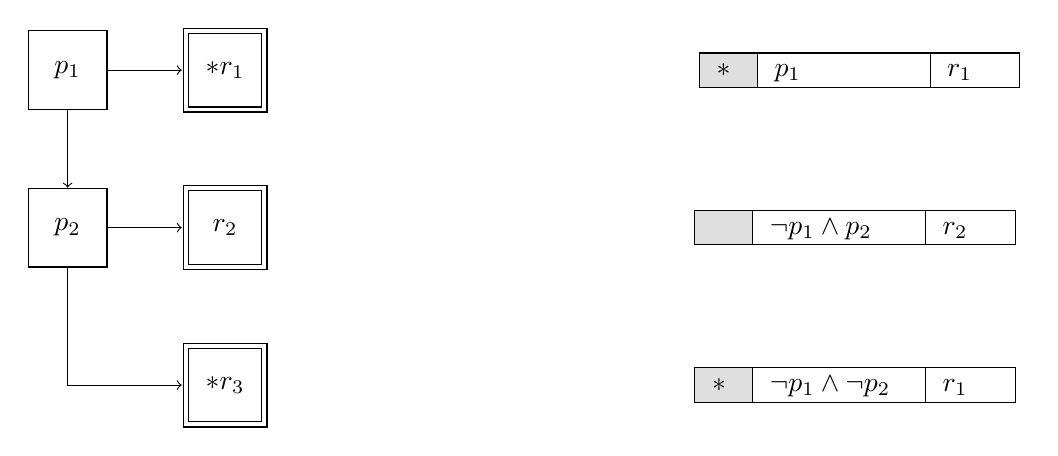
\begin{tikzpicture}[x=20mm, y=20mm]
\tikzset{Pred/.style={shape=rectangle, draw, minimum width=1cm, minimum height=1cm}}
\tikzset{Res/.style={shape=rectangle, draw, double distance=0.5mm, outer sep=0.5mm, minimum width=1cm, minimum height=1cm}}

% nodes
\node[Pred] (p1) at (0, 2) {$p_1$};
\node[Res]  (r1) at (1, 2) {$\ast r_1$};
\node (case1) at (5, 2) {
{}
\begin{tabular}{|p{3mm}|p{5em}|p{2em}|}\hline
\cellcolor{gray!25} $\ast$ & $p_1$ & $r_1$\\\hline
\end{tabular}};

\node[Pred] (p2) at (0, 1) {$p_2$};
\node[Res] (r2) at (1, 1) {$r_2$};
\node (case1) at (5, 1) {\begin{tabular}{|p{3mm}|p{5em}|p{2em}|}\hline
\cellcolor{gray!25} ~~ & $\neg p_1 \land p_2$ & $r_2$\\\hline
\end{tabular}};

\node[Res] (r3) at (1, 0) {$\ast r_3$};
\node (case1) at (5, 0) {\begin{tabular}{|p{3mm}|p{5em}|p{2em}|}\hline
\cellcolor{gray!25} $\ast$ & $\neg p_1 \land \neg p_2$ & $r_1$\\\hline
\end{tabular}};
% arrows
\draw[->] (p1) -> (r1);
\draw[->] (p1) -- (p2);
\draw[->] (p2) -- (r2);
\draw[->] (p2) |- (r3);
\end{tikzpicture}

\iffalse
\begin{tabular}{|r|rrr|r|}\hline
$\ast$ &      $p_1$ &         &            & $r_1$ \\\hline
       & $\neg p_1$ & $\land$ &      $p_2$ & $r_2$ \\\hline
$\ast$ & $\neg p_1$ & $\land$ & $\neg p_2$ & $r_3$      \\\hline
\end{tabular}
\fi

\subsection{Recursive \WHEN's}
Recursive predicates cannot be solved and are therefore considered as part of the result (recursive) expression. Slicing stops before a recursive predicate.

\begin{tikzpicture}[x=20mm, y=20mm]
\tikzset{Pred/.style={shape=rectangle, draw, minimum width=1cm, minimum height=1cm}}
\tikzset{Res/.style={shape=rectangle, draw, double distance=0.5mm, outer sep=0.5mm, minimum width=1cm, minimum height=1cm}}

% nodes
\node[Pred] (p1) at (0, 1.5) {$p_1$};
\node[Res]  (r1) at (1, 1.5) {$r_1$};
\node at (5, 1.5) {\begin{tabular}{|p{3mm}|p{5em}|p{2em}|}\hline
\cellcolor{gray!25} & $p_1$ & $r_1$\\\hline
\end{tabular}};

\node[Res, inner sep=3mm] (res) at (0.5, 0) {
    \begin{tikzpicture}[x=20mm, y=20mm, inner sep=1em]
        \node[Pred] (p2) at (0, 1) {$\ast p_2$};
        \node[Pred] (r2) at (1, 1) {$r_2$};
        \node[Pred] (r3) at (1, 0) {$r_3$};
        \draw[->] (p2) -- (r2);
        \draw[->] (p2) |- (r3);
    \end{tikzpicture}
};
\node at (5, 0) {\begin{tabular}{|c|c|c|}\hline
\cellcolor{gray!25} $\ast$ & $\neg p_1$ & $\WHEN ~p_2~ \THEN ~r_1~ \ELSE ~r_3$\\\hline
\end{tabular}};
% arrows
\draw[->] (p1) -> (r1);
\draw[->] (p1) -> (0, 0.95);
\end{tikzpicture}

\subsection{Nonrecursive subtrees}
Subtrees with no callsite are taken as one big basecase without further slicing.

\begin{tikzpicture}[x=20mm, y=20mm]
\tikzset{Pred/.style={shape=rectangle, draw, minimum width=1cm, minimum height=1cm}}
\tikzset{Res/.style={shape=rectangle, draw, double distance=0.5mm, outer sep=0.5mm, minimum width=1cm, minimum height=1cm}}

% nodes
\node[Pred] (p1) at (0, 1.5) {$p_1$};
\node[Res]  (r1) at (1, 1.5) {$\ast r_1$};
\node at (5, 1.5) {\begin{tabular}{|p{3mm}|p{5em}|p{2em}|}\hline
\cellcolor{gray!25} $\ast$ & $p_1$ & $r_1$\\\hline
\end{tabular}};

\node[Res, inner sep=3mm] (res) at (0.5, 0) {
    \begin{tikzpicture}[x=20mm, y=20mm, inner sep=1em]
        \node[Pred] (p2) at (0, 1) {$p_2$};
        \node[Pred] (r2) at (1, 1) {$r_2$};
        \node[Pred] (r3) at (1, 0) {$r_3$};
        \draw[->] (p2) -- (r2);
        \draw[->] (p2) |- (r3);
    \end{tikzpicture}
};
\node at (5, 0) {\begin{tabular}{|c|c|c|}\hline
\cellcolor{gray!25} ~~ & $\neg p_1$ & $\WHEN ~p_2~ \THEN ~r_1~ \ELSE ~r_3$\\\hline
\end{tabular}};
% arrows
\draw[->] (p1) -> (r1);
\draw[->] (p1) -> (0, 0.95);
\end{tikzpicture}

\subsection{Nested Case in \THEN}
Predicates stack up linearily when nested inside \THEN.

\begin{tikzpicture}[x=15mm, y=15mm]
\tikzset{Pred/.style={shape=rectangle, draw, minimum width=1cm, minimum height=1cm}}
\tikzset{Box/.style={shape=rectangle, draw, minimum width=1cm, minimum height=1cm, dotted, very thick}}
\tikzset{Res/.style={shape=rectangle, draw, double distance=0.5mm, outer sep=0.5mm, minimum width=1cm, minimum height=1cm}}

% nodes
\node[Pred] (p) at (0, 1) {$p$};
\node[Box]  (r1) at (2, 1) {
    \begin{tikzpicture}[x=15mm, y=15mm]
        \node[Pred] (p1) at (0, 2.5) {$p_1$};
        \node[Res] (r1) at (1, 2.5) {$r_1$};
        
        \node[Pred] (pi) at (0, 1) {$p_i$};
        \node[Res] (ri) at (1, 1) {$r_i$};
        % arrows
        \draw[->] (p1) -- (r1);
        \draw[->] (pi) -- (ri);
        \draw[->, dash pattern=on 5pt off 1pt on 3pt off 3pt on 1pt off 2pt on 1pt off 2pt on 3pt off 1pt] (p1) -- (pi);
        \draw[->, dash pattern=on 5pt off 1pt on 3pt off 3pt on 1pt off 2pt on 1pt off 2pt on 3pt off 1pt] (pi) -- +(0,-1);
    \end{tikzpicture}
};
\node at (5, 2) {
    \begin{tabular}{|p{1em}|p{3cm}|c|}\hline
    \cellcolor{gray!25}  & $p \land \phantom{\neg}p_1 $& $r_1$\\\hline
    \end{tabular}
};
   
\node at (5, 1.4) { 
    \vdots
};
    
\node at (5, 0.65) {
    \begin{tabular}{|p{1em}|p{3cm}|c|}\hline
    \cellcolor{gray!25}  & $p \land \neg p_1 \land \neg p_2 \land \hdots \land p_i$& $r_2$\\\hline
    \end{tabular}
};
% arrows
\draw[->] (p) -- (r1);
\end{tikzpicture}


\iffalse
\begin{tabular}{lllrrrrrrrrrr}
\WHEN ~$p_1$~ \THEN & &                        &         $r_1$&  &$\Rightarrow$ (&     $p_1$ &       &           &         &               &                    &, $r_1$)\\
\WHEN ~$p_2$~ \THEN &(&\WHEN ~$p_{2,1}$~ \THEN &     $r_{2,1}$&  &$\Rightarrow$ (&$\neg p_1$ &$\land$&     $ p_2$& $\land$ &    $ p_{2,1}$ &                    &, $r_{2,1}$)\\
                    & &\WHEN ~$p_{2,2}$~ \THEN &     $r_{2,2}$&  &$\Rightarrow$ (&$\neg p_1$ &$\land$&     $ p_2$& $\land$ &$\neg p_{2,1}$ &                    &, $r_{2,2}$)\\
                    & &\ELSE                   &$\ast r_{2,3}$&) &$\Rightarrow$ (&$\neg p_1$ &$\land$&     $ p_2$& $\land$ &$\neg p_{2,1}$ &$\land \neg p_{2,2}$&, $r_{2,1}$)\\
\ELSE               & &                        &    $\ast r_3$&  &$\Rightarrow$ (&$\neg p_1$ &$\land$& $\neg p_2$&         &               &                    &, $r_3$)\\
\end{tabular}
\fi


\subsection{Nested Case in \WHEN's}
When \CASE-expressions are nested inside \WHEN, there two ways not to receive a given result.

\begin{tikzpicture}[x=15mm, y=15mm]
\tikzset{Pred/.style={shape=rectangle, draw, minimum width=1cm, minimum height=1cm}}
\tikzset{Box/.style={shape=rectangle, draw, minimum width=1cm, minimum height=1cm, dotted, very thick}}
\tikzset{Res/.style={shape=rectangle, draw, double distance=0.5mm, outer sep=0.5mm, minimum width=1cm, minimum height=1cm}}


% nodes
\node[Pred] (p) at (0, 3) {$p$};

\node[Box] (p1) at (0, 1) {
    \begin{tikzpicture}[x=15mm, y=15mm]
        \node[Pred] (p2) at (0, 1) {$\pi_i$};
        \node[Pred] (r2) at (1, 1) {$p_i$};
        % arrows
        \draw[->] (p2) -- (r2);
        \draw[->] (r2) -- +(0, -1);
        \draw[<-, dash pattern=on 5pt off 1pt on 3pt off 3pt on 1pt off 2pt on 1pt off 2pt on 3pt off 1pt] (p2) -- +(0,1);
        \draw[->, dash pattern=on 5pt off 1pt on 3pt off 3pt on 1pt off 2pt on 1pt off 2pt on 3pt off 1pt] (p2) -- +(0,-1);
    \end{tikzpicture}
};
\node[Res] (r1) at (2, 1) {$\ast r_i$};
\node (case1) at (4, 1) {
    \begin{tabular}{|p{1em}|r|c|}\hline
    \cellcolor{gray!25} $\ast$ & $\neg p \land \pi_i \land p_i$ & $r_i$\\\hline
    \end{tabular}
};

\node[Res] (r) at (0, -1) {$\ast r$};
\node (case1) at (4, -1) {
    \begin{tabular}{|p{1em}|rrr|c|}\hline
    \cellcolor{gray!25} $\ast$ & $\neg p \land$ & $     \pi_i$ & $\land \neg p_i$ & $r$\\\hline
    \cellcolor{gray!25} $\ast$ & $\neg p \land$ & $\neg \pi_i$ &                  & $r$\\\hline
    \end{tabular}
};
% arrows
\draw[->] (p) -- (p1);
\draw[->] (p1) -- (r1);
\draw[->] (p1) -- (r);
\end{tikzpicture}

\subsection{\CASE- and \ELSE-rules}
\begin{prooftree}
    \AxiomC{}\RightLabel{\scriptsize(base)}
    \UnaryInfC{\lstinputlisting{snippets/rules/fib/03-case-when.sql}}
    \AxiomC{}\RightLabel{\scriptsize(base)}
    \UnaryInfC{\lstinputlisting{snippets/rules/fib/03-case-then.sql}}
    \AxiomC{\vdots}\RightLabel{\scriptsize(else)}
    \UnaryInfC{\lstinputlisting{snippets/rules/fib/03-case-else.sql}}
    \RightLabel{\scriptsize(when)}
    \TrinaryInfC{\lstinputlisting{snippets/rules/fib/02-case.sql}}
\end{prooftree}


$$\quad(\textsc{when})\inferrule{
    \neg (\hasCallsite(p) \land \hasCallsite(bs))\\
    T, C \vdash (\TRUE, p) \rightarrow (B_p, R_p) \\
    T, C \vdash (\TRUE, e) \rightarrow (B_e, R_e)\\
    B_p = \{(p_{p_1}, p'_1), ..., (p_{p_n}, p'_n)\} \\
    \forall (p_{p_i}, p'_i) \in B_p: T, C \vdash (p_0 ~\AND~ p_{p_i}~\AND~\NOT~ p'_i,~ \CASE bs \END) \rightarrow (B_i, R_i) \\
}{
    T, C \vdash (p_0, \CASE \WHEN p \THEN e ~bs \END) \rightarrow \\\\
    {\begin{tabular}[b]{LLLLLL}
        (&\{&(p_0 ~\AND~ p_p ~\AND~ p' ~\AND~ p_e &, e'&) ~|~~(p_p, p') \in B_p, (p_e, e') \in B_e \} &~\cup~ (\cup_{1\leq i \leq n}B_i), \\
         &\{&(p_0 ~\AND~ p_p ~\AND~ p' ~\AND~ p_e &, e'&) ~|~~(p_p, p') \in B_p, (p_e, e') \in R_e \}&~\cup~ (\cup_{1\leq i \leq n}R_i) ~\cup \\
         &\{&(p_0 ~\AND~ p_p ~\AND~ p_0             &, \CASE \WHEN p'_1 \THEN e ~bs \END&) ~|~~(p_p, p') \in R_p \})
    \end{tabular}}
}$$

$$\quad(\textsc{else})\inferrule{
    T, C \vdash (p, e) \rightarrow (B, R) \\
}{
    T, C \vdash (p, \CASE \ELSE e \END) \rightarrow (B, R)
}$$

\section{Handling recursive operands}

\begin{figure}
    \centering
    
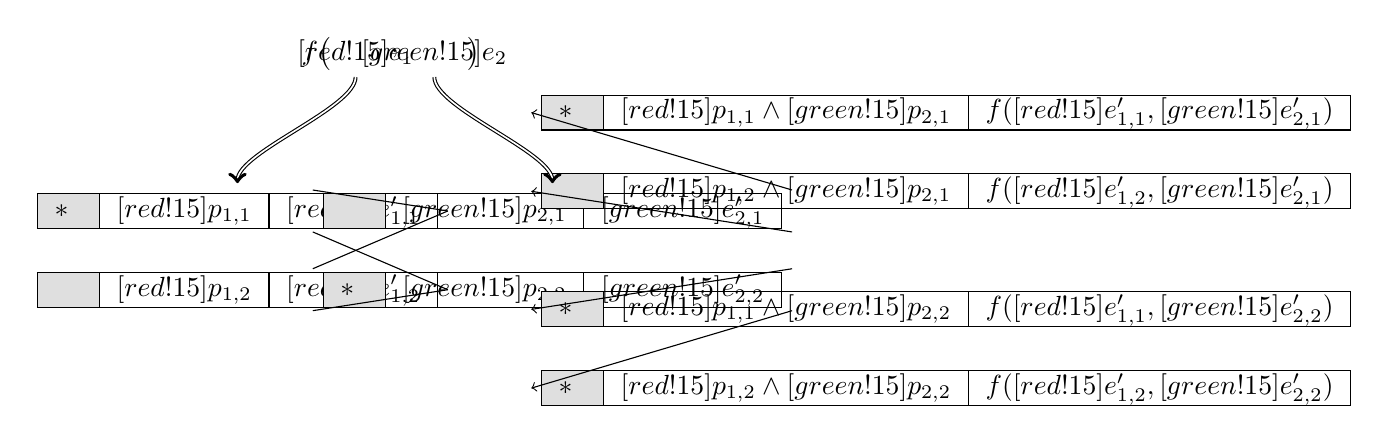
\begin{tikzpicture}[x=10mm, y=10mm]
\node      at (1, 5) {$f\big($};
\node (e1) at (1.5, 5) {$\highlight[red!15]{e_1}$};
\node      at (2, 5) {$,$};
\node (e2) at (2.5, 5) {$\highlight[green!15]{e_2}$};
\node      at (3, 5) {$\big)$};

\node (e11) at (0, 3) { 
    \begin{tabular}{|p{1em}|r|c|}\hline
    \cellcolor{gray!25} $\ast$ & $\highlight[red!15]{p_{1,1}}$ & $\highlight[red!15]{e'_{1,1}}$\\\hline
    \end{tabular}
};
\node (e12) at (0, 2) { 
    \begin{tabular}{|p{1em}|r|c|}\hline
    \cellcolor{gray!25}  & $\highlight[red!15]{p_{1,2}}$ & $\highlight[red!15]{e'_{1,2}}$\\\hline
    \end{tabular}
};

\node (e21) at (4, 3) { 
    \begin{tabular}{|p{1em}|r|c|}\hline
    \cellcolor{gray!25}  & $\highlight[green!15]{p_{2,1}}$ & $\highlight[green!15]{e'_{2,1}}$\\\hline
    \end{tabular}
};
\node (e22) at (4, 2) { 
    \begin{tabular}{|p{1em}|r|c|}\hline
    \cellcolor{gray!25}$\ast$ & $\highlight[green!15]{p_{2,2}}$ & $\highlight[green!15]{e'_{2,2}}$\\\hline
    \end{tabular}
};

\node (r1) at (9, 4.25) { 
    \begin{tabular}{|p{1em}|r|c|}\hline
    \cellcolor{gray!25} $\ast$ & $\highlight[red!15]{p_{1,1}} \land \highlight[green!15]{p_{2,1}}$ & $f(\highlight[red!15]{e'_{1,1}}, \highlight[green!15]{e'_{2,1}})$\\\hline
    \end{tabular}
};
\node (r2) at (9, 3.25) { 
    \begin{tabular}{|p{1em}|r|c|}\hline
    \cellcolor{gray!25}  & $\highlight[red!15]{p_{1,2}} \land \highlight[green!15]{p_{2,1}}$ & $f(\highlight[red!15]{e'_{1,2}}, \highlight[green!15]{e'_{2,1}})$\\\hline
    \end{tabular}
};

\node (r3) at (9, 1.75) { 
    \begin{tabular}{|p{1em}|r|c|}\hline
    \cellcolor{gray!25} $\ast$ & $\highlight[red!15]{p_{1,1}} \land \highlight[green!15]{p_{2,2}}$ & $f(\highlight[red!15]{e'_{1,1}}, \highlight[green!15]{e'_{2,2}})$\\\hline
    \end{tabular}
};
\node (r4) at (9, 0.75) { 
    \begin{tabular}{|p{1em}|r|c|}\hline
    \cellcolor{gray!25} $\ast$ & $\highlight[red!15]{p_{1,2}} \land \highlight[green!15]{p_{2,2}}$ & $f(\highlight[red!15]{e'_{1,2}}, \highlight[green!15]{e'_{2,2}})$\\\hline
    \end{tabular}
};
\draw[->, double, out=270, in=90, looseness = 0.5] (e1.south) to (e11);
\draw[->, double, out=270, in=90, looseness = 0.5] (e2.south) to (e21);

\draw (e11.east) -- (e21.175);
\draw (e11.east) -- (e22.175);
\draw (e12.east) -- (e21.185);
\draw (e12.east) -- (e22.185);

\draw[->] (e21.5) -- (r1.west);
\draw[->] (e21.355) -- (r2.west);
\draw[->] (e22.5) -- (r3.west);
\draw[->] (e22.355) -- (r4.west);
\end{tikzpicture}

    \caption{Operands of a function are translated separately. For each operand a number of scenarios is generated. All possible scenarios of the original function are created by using the cross product.}
    \label{fig:expr-expr}
\end{figure}

\subsection{Single recursive operand}
\subsection{Multiple recursive operands}
\subsection{EXPR-Rule}
$
\inferrule*[Right=(expr)]{
    \inferrule*[Left=(rec)]{ }{
        {\begin{minipage}[b]{15em}
        \mintinline{postgresql}{(TRUE, fib($1 - 1)) ->}
        \mintinline{postgresql}{({}, {(TRUE, fib($1 - 1))})}
        \end{minipage}}
    }\\
    \inferrule*[Right=(rec)]{ }{
        {\begin{minipage}[b]{15em}
        \mintinline{postgresql}{(TRUE, fib($1 - 2)) ->}
        \mintinline{postgresql}{({}, {(TRUE, fib($1 - 2))})}
        \end{minipage}}
    }
}{
    {\begin{minipage}[b]{25em}
    \mintinline{postgresql}{(TRUE, fib($1 - 1) + fib($1 - 2)) ->}
    \mintinline{postgresql}{({}, {(TRUE AND TRUE AND TRUE, fib($1 - 1) + fib($1 - 2))})}
    \end{minipage}}
}
$

$$\quad(\textsc{expr})\inferrule{
    \exists i \in \{1, ..., n\}: T \vdash \hasCallsite(e_i)\\
    \forall i \in \{1, ..., n\}: T, C \vdash (\TRUE, e_i) \rightarrow (B_i, R_i)
}{
    T, C \vdash (p, \oplus_{1\leq i \leq n} e_i) \rightarrow \\\\
    {\begin{tabular}[b]{LLL}
        (&\{(p ~\AND~ (\AND_{1\leq i \leq n} p_i)), \oplus_{1\leq i \leq n} e_i' &~|~~ ((p_1, e_1'), ..., (p_n, e_n')) \in \times_{\{i|1\leq i \leq n\}} ~B_i\}, \\
        &\{(p ~\AND~ (\AND_{1\leq i \leq n } p_i)), \oplus_{1\leq i \leq n} e_i &~|~~ ((p_1, e_1'), ..., (p_n, e_n')) \in \times_{\{i|1\leq i \leq n\}} (B_i \cup R_i),\\&&~~~~\exists e \in \{e'_1, ..., e'_n\} : \hasCallsite(T, e)\})
    \end{tabular}}
}$$
\\


\subsection{\RSELECT- and \RFROM-rule}
\begin{figure}
    \centering
    {\small
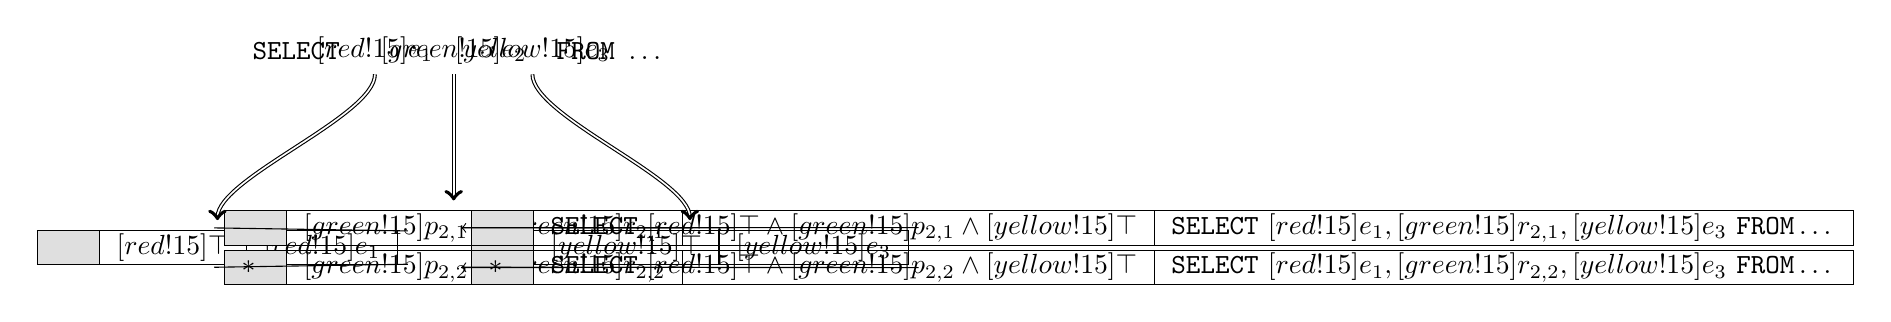
\begin{tikzpicture}[x=5mm, y=5mm]
\node      at ( 8, 9) {$\SELECT$};
\node (e1) at (10, 9) {$\highlight[red!15]{e_1}$};
\node      at (11, 9) {$,$};
\node (e2) at (12, 9) {$\highlight[green!15]{e_2}$};
\node      at (13, 9) {$,$};
\node (e3) at (14, 9) {$\highlight[yellow!15]{e_3}$};
\node      at (16, 9) {$\FROM ~ \dots$};

\node (e11) at (6, 4) { 
    \begin{tabular}{|p{1em}|r|c|}\hline
    \cellcolor{gray!25}  & $\highlight[red!15]{\top}$ & $\highlight[red!15]{e_1}$\\\hline
    \end{tabular}
};

\node (e21) at (12, 4.5) { 
    \begin{tabular}{|p{1em}|r|c|}\hline
    \cellcolor{gray!25}  & $\highlight[green!15]{p_{2,1}}$ & $\highlight[green!15]{r_{2,1}}$\\\hline
    \end{tabular}
};
\node (e22) at (12, 3.5) { 
    \begin{tabular}{|p{1em}|r|c|}\hline
    \cellcolor{gray!25} $\ast$ & $\highlight[green!15]{p_{2,2}}$ & $\highlight[green!15]{r_{2,2}}$\\\hline
    \end{tabular}
};

\node (e31) at (18, 4) { 
    \begin{tabular}{|p{1em}|r|c|}\hline
    \cellcolor{gray!25} & $\highlight[yellow!15]{\top}$ & $\highlight[yellow!15]{e_3}$\\\hline
    \end{tabular}
};

\node (r1) at (30, 4.5) { 
    \begin{tabular}{|p{1em}|r|c|}\hline
    \cellcolor{gray!25}  & $\SELECT ~ \highlight[red!15]{\top} \land \highlight[green!15]{p_{2,1}} \land \highlight[yellow!15]{\top}$ & $\SELECT~ \highlight[red!15]{e_1}, \highlight[green!15]{r_{2,1}}, \highlight[yellow!15]{e_3} ~ \FROM \dots$\\\hline
    \end{tabular}
};
\node (r2) at (30, 3.5) { 
    \begin{tabular}{|p{1em}|r|c|}\hline
    \cellcolor{gray!25} $\ast$ & $\SELECT ~ \highlight[red!15]{\top} \land \highlight[green!15]{p_{2,2}} \land \highlight[yellow!15]{\top}$ & $\SELECT~ \highlight[red!15]{e_1}, \highlight[green!15]{r_{2,2}}, \highlight[yellow!15]{e_3} ~ \FROM \dots$\\\hline
    \end{tabular}
};
\draw[->, double, out=270, in=90, looseness = 0.5] (e1.south) to (e11);
\draw[->, double, out=270, in=90, looseness = 0.5] (e2.south) to (e21);
\draw[->, double, out=270, in=90, looseness = 0.5] (e3.south) to (e31);
\draw (e11.5) to (e21.west);
\draw (e11.355) to (e22.west);
\draw (e21.east) to (e31.175);
\draw (e22.east) to (e31.185);
\draw[->] (e31.5) -- (r1.west);
\draw[->] (e31.355) -- (r2.west);
%\draw[->, bend left=20]  (e11.north) to (e21.north) to (e31.north) to (r1.west);
%\draw[->, bend right=20] (e11.south) to (e22.south) to (e31.south) to (r2.west);
\end{tikzpicture}}
    \caption{The projection of a relation happening inside \SELECT~can be viewed as a function with a number of operands, ie. the output columns. The same happens analogiously for the \FROM-clause.}
    \label{fig:expr-select}
\end{figure}

\subsection{\RSELECT- and \RFROM-rule}
\begin{figure}
    \centering
    {\small
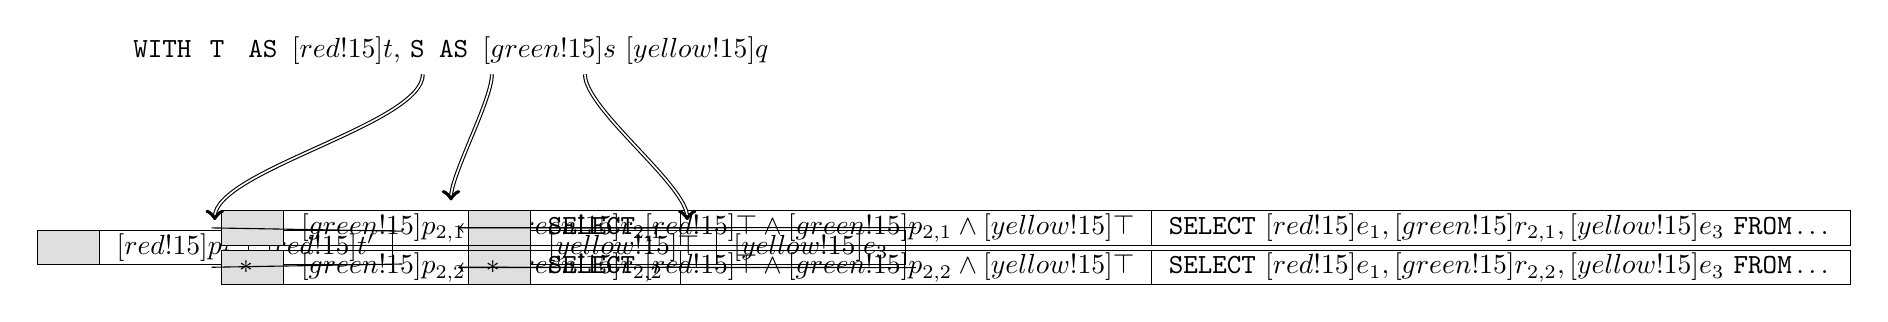
\begin{tikzpicture}[x=5mm, y=5mm, node distance=1mm]
\node (ctes) at (12,9) {\WITH~ \texttt{T} \AS $\highlight[red!15]{t}$, \texttt{S}\AS $\highlight[green!15]{s}$ $\highlight[yellow!15]{q}$};

\node (e11) at (6, 4) { 
    \begin{tabular}{|p{1em}|r|c|}\hline
    \cellcolor{gray!25}  & $\highlight[red!15]{p_t}$ & $\highlight[red!15]{t'}$\\\hline
    \end{tabular}
};

\node (e21) at (12, 4.5) { 
    \begin{tabular}{|p{1em}|r|c|}\hline
    \cellcolor{gray!25}  & $\highlight[green!15]{p_{2,1}}$ & $\highlight[green!15]{r_{2,1}}$\\\hline
    \end{tabular}
};
\node (e22) at (12, 3.5) { 
    \begin{tabular}{|p{1em}|r|c|}\hline
    \cellcolor{gray!25} $\ast$ & $\highlight[green!15]{p_{2,2}}$ & $\highlight[green!15]{r_{2,2}}$\\\hline
    \end{tabular}
};

\node (e31) at (18, 4) { 
    \begin{tabular}{|p{1em}|r|c|}\hline
    \cellcolor{gray!25} & $\highlight[yellow!15]{\top}$ & $\highlight[yellow!15]{e_3}$\\\hline
    \end{tabular}
};

\node (r1) at (30, 4.5) { 
    \begin{tabular}{|p{1em}|r|c|}\hline
    \cellcolor{gray!25}  & $\SELECT ~ \highlight[red!15]{\top} \land \highlight[green!15]{p_{2,1}} \land \highlight[yellow!15]{\top}$ & $\SELECT~ \highlight[red!15]{e_1}, \highlight[green!15]{r_{2,1}}, \highlight[yellow!15]{e_3} ~ \FROM \dots$\\\hline
    \end{tabular}
};
\node (r2) at (30, 3.5) { 
    \begin{tabular}{|p{1em}|r|c|}\hline
    \cellcolor{gray!25} $\ast$ & $\SELECT ~ \highlight[red!15]{\top} \land \highlight[green!15]{p_{2,2}} \land \highlight[yellow!15]{\top}$ & $\SELECT~ \highlight[red!15]{e_1}, \highlight[green!15]{r_{2,2}}, \highlight[yellow!15]{e_3} ~ \FROM \dots$\\\hline
    \end{tabular}
};
\draw[->, double, out=270, in=90, looseness = 0.5] (ctes.220) to (e11);
\draw[->, double, out=270, in=90, looseness = 0.5] (ctes.330) to (e21);
\draw[->, double, out=270, in=90, looseness = 0.5] (ctes.350) to (e31);
\draw (e11.5) to (e21.west);
\draw (e11.355) to (e22.west);
\draw (e21.east) to (e31.175);
\draw (e22.east) to (e31.185);
\draw[->] (e31.5) -- (r1.west);
\draw[->] (e31.355) -- (r2.west);
%\draw[->, bend left=20]  (e11.north) to (e21.north) to (e31.north) to (r1.west);
%\draw[->, bend right=20] (e11.south) to (e22.south) to (e31.south) to (r2.west);
\end{tikzpicture}}
    \caption{The projection of a relation happening inside \SELECT~can be viewed as a function with a number of operands, ie. the output columns. The same happens analogiously for the \FROM-clause.}
    \label{fig:expr-select}
\end{figure}

If the callsites of a query a located in the \FROM-part, it means that at least one table referenced is recursive, ie. contains a callsite or a reference a recursive table. 
As the tables within the same \FROM cannot reference each other, we can process each table independently and resemble the whole query with all possible combinations, similar to the \REXPR-rule. For an example see this example:
\sqlcode[mathescape=true]{snippets/rule_from_example.sql}


$
\inferrule*{
    \inferrule*{...}{
{\begin{minipage}[b]{12em}
\sqlcode{snippets/rules/fib/01-case.sql}
\end{minipage}}
    }
}{
{\begin{minipage}[b]{12em}
\sqlcode{snippets/rules/fib/01-select.sql}
\end{minipage}}
}
$


$$\quad(\textsc{select})\inferrule{
    \exists i \in \{1, ..., k\}: T \vdash \hasCallsite(e_{s_i}) \\
    \forall i \in \{1 \leq i \leq n\} : T \vdash \neg \hasCallsite(e_{t_i}) \\
    T \vdash \neg \hasCallsite(e_{w}) \\
    \forall i \in \{1, ..., k\}: T, \varnothing \vdash (\TRUE, e_{s_i}) \rightarrow (B_i, R_i)
}{
    T, \varnothing \vdash (p, \SELECT [\texttt{DISTINCT}]~ e_{s_1}, ..., e_{s_k} \FROM t_1 \AS a_1 \otimes ... \otimes  t_n \AS a_n \WHERE e_w) \rightarrow \\\\
    {\begin{tabular}[b]{LLLL}
    (~~&\{&(&\SELECT p ~\AND~ p_{s_1} ~\AND~ \cdots ~\AND~ p_{s_k},\\
        &&&\SELECT [\texttt{DISTINCT}]~ e'_{s_1}, ..., e'_{s_k} \FROM t_1 \AS a_1 \otimes ... \otimes  t_n \AS a_n \WHERE e_w~~) \\
        && | &~((p_{s_1}, e'_{s_1}), ..., (p_{s_k}, e'_{s_k})) \in \times_{1 \leq i \leq k} B_i~~\}, \\
     &\{&(&\SELECT p ~\AND~ p_{s_1} ~\AND~ \cdots ~\AND~ p_{s_k}, \\
        &&&\SELECT [\texttt{DISTINCT}]~ e'_{s_1}, ..., e'_{s_k} \FROM t_1 \AS a_1 \otimes ... \otimes  t_n \AS a_n \WHERE e_w~~) \\
        && | &~((p_{s_1}, e'_{s_1}), ..., (p_{s_k}, e'_{s_k})) \in \times_{1 \leq i \leq k} (B_i \cup R_i), \exists e \in \{e'_{s_1}, ..., e'_{s_k}\} : \hasCallsite(e)~~\}~~)\\
    \end{tabular}}
}$$
\subsection{WHERE-Rule}
$$\quad(\textsc{where})\inferrule{
    T \vdash \neg \hasCallsite(e_{s}) \\
    \forall i \in \{1 \leq i \leq n\} : T \vdash \neg \hasCallsite(e_{t_i}) \\
    T \vdash \hasCallsite(e_{w}) \\
    T, \varnothing \vdash (p, e_{w}) \rightarrow (B, R)
}{
    T, \varnothing \vdash (p, \SELECT e_s \FROM t_1 \AS a_1 \otimes ... \otimes  t_n \AS a_n \WHERE e_w) \rightarrow \\\\
    {\begin{tabular}[b]{LLLL}
    (~~&\{&(&\SELECT p_w  \FROM t_1 \AS a_1 \otimes ... \otimes  t_n \AS a_n \WHERE e'_w,\\
        &&&\SELECT e_s \FROM t_1 \AS a_1 \otimes ... \otimes  t_n \AS a_n \WHERE e'_w~~) \\
        && | &~(p_w, e'_w) \in B~~\}, \\
     &\{&(&\SELECT p_w \FROM t_1 \AS a_1 \otimes ... \otimes  t_n \AS a_n \WHERE e'_w, \\
        &&&\SELECT e_s \FROM t_1 \AS a_1 \otimes ... \otimes  t_n \AS a_n \WHERE e'_w~~) \\
        && | &~(p_w, e'_w) \in R~~\}~~)\\
    \end{tabular}}
}$$
\\
\section{Handling CTEs}

The notion of \textit{containing a callsite} (or being \textit{recursive}) is simple when considering only S-F-W queries. If a sql-fragment $e$ contains a callsite, the subexpression is recursive: $\hasCallsite(e) = fn \sqsubset e$. From an implementation point of view, it is as simple as filtering the AST of $e$ for callsites.

\begin{wrapfigure}{r}{.5\textwidth}
    \begin{minipage}{\linewidth}
    \centering \captionsetup[subfigure]{justification=centering}
    \begin{minted}{sql}
    WITH T AS (SELECT f(n-1))
    SELECT * FROM T
    \end{minted}
    \subcaption{The actual query contains no direct callsite. Yet, it is still recursive since it references a recursive CTE.}
    \label{fig:simple_indiref}\par\vfill
    \begin{minted}{sql}
    WITH S AS (SELECT f(n-1)),
         T AS (SELECT * FROM S)
    SELECT * FROM T
    \end{minted}
    \subcaption{Neither the actual query nor the referenced CTE \texttt{T} directly contains a callsite.}
    \label{fib_nonrec_scenarios}\par\vfill
    \begin{minted}{sql}
    SELECT (
        WITH T AS (SELECT f(n-1))
        SELECT 1
    )
    \end{minted}
    \subcaption{Our definition of $\hasCallsite$ would fail here since a callsite is located in the subtree. The query is acutally nonrecursive.}
    \label{fig:trimmed_ref}
\end{minipage}
\caption{}
\label{lst:indirect_callsite_ref}
\end{wrapfigure}

With CTEs we need to take into account two things. First, callsites can now be located outside the current subtree (\autoref{fig:simple_indiref}). Second, the scenario may contain unused recursive CTEs (\autoref{fig:trimmed_ref}), fooling $\hasCallsite$ stated above to believe a given SQL-fragment is recursive, even if the recursive CTEs are never evaluated.

We can work around this issues, if we remove the CTEs from the original query before translating the actual query. For each query-scenario only those CTEs are reattached afterwards, that are actually used (\autoref{tracking_recursive_ctes}). To detect indirect callsite references, we note recursive CTEs when detaching (\autoref{tracking_cte_dependencies}).

\subsection{Tracking recursive CTEs}\label{tracking_recursive_ctes}

To address this circumstances, the inference rules are extended with an environment $(T, C)$. It consists of the set of recursive table-variables in scope, $T$, and a list $C$ of CTE-scenarios. 

This queue is used when the CTEs are processed and then removed from the query until the actual query is translated and the used CTEs are known.

Each CTE-scenario is augmented with its dependencies to previously defined CTEs. Each CTE is sliced into its different scenarios, then each scenario is analyzed, removed from the query and stored in the queue. When all CTEs are processed and the actual query is translated, only those CTEs are reattached to the query-scenario that are actually used. Indirect callsites can be detected by simply checking if there exists a free table-variable that is enlisted in $T$.

To address the detection of indirect callsites, we need to keep track of recursive table-variables in scope. We will use a simple set $T$ which contains all recursive table-variables in scope. $\hasCallsite$ will then check additionally if any variable of $T$ is used in a subexpression:
\begin{align*}
    \hasCallsite(T, e) =& fn(\dots) \sqsubset e \lor FV(e) \cap T \neq \emptyset
\end{align*}
The function $\FV$ computes all the free table-variables of a sql-fragment. It is implemented straight forward: Each CTE definition within a \WITH-block adds its alias to the list of bound table-variables. Every reference to a table-variable that is not contained in that list is considered free.

% Row-references vs. table-variables
Note that there can occur two different types of free variables inside a given subexpression: \textit{Table-Variables} and \textit{Row-References}. Table-variables like \texttt{T} are used exclusively in ~\FROM~ and reference an entire table. This table-variables are introduced either by the existance of a table in the current database or by an CTE. On the other hand, row-references like \texttt{T.v} point to a single table-row in each iteration through the intermediate (eg. join-)table of the \FROM-clause\footnote{Actually, only \texttt{T} is the row-reference and \texttt{.v} is a selector of the column \texttt{v} from that row.}).

Row-references are considered therefore always nonrecursive, as they are eventually bound by a ~\FROM~ that links that reference to a table-variable. If a query uses a recursive table-variable, those recursive calls are evaluated \textit{before} the variables are bound. The row-references used in ~\SELECT~ and ~\WHERE~ are thus just reference to an intermediate result, that is not recursive anymore. Also, even if no row-reference is used at all, the recursive table-variables are processed anyway. Therefore it is sufficient to track only table-variables.
\\




Now we can formalize the notion of \textit{containing a callsite}, if we assume a set $T$ of recursive table-variables in the current scope and the name of the recursive UDF $fn$ are given. The function $FV(e)$ computes a set of all free table-variables within $e$.

%An expression is considered recursive if it contains directly a recursive call or references a recursive table-variable.

%Table-Variable vs. Row-References
%- CTEs creates new table-variables
%- FROMs use table-variables to create new row-references



Instead of tracing every reference through the entire query until the initial definition is found, we take an incremental approach: If a new table-variable is created, we check each free variable in its subtree against the environment of known recursive table-references within that scope. If there is a recursive table referenced or the subtree contains an immediate recursive call, the new table-reference is entailed the set of recursive table-references.



\begin{figure}[h]
    \small
    \centering
    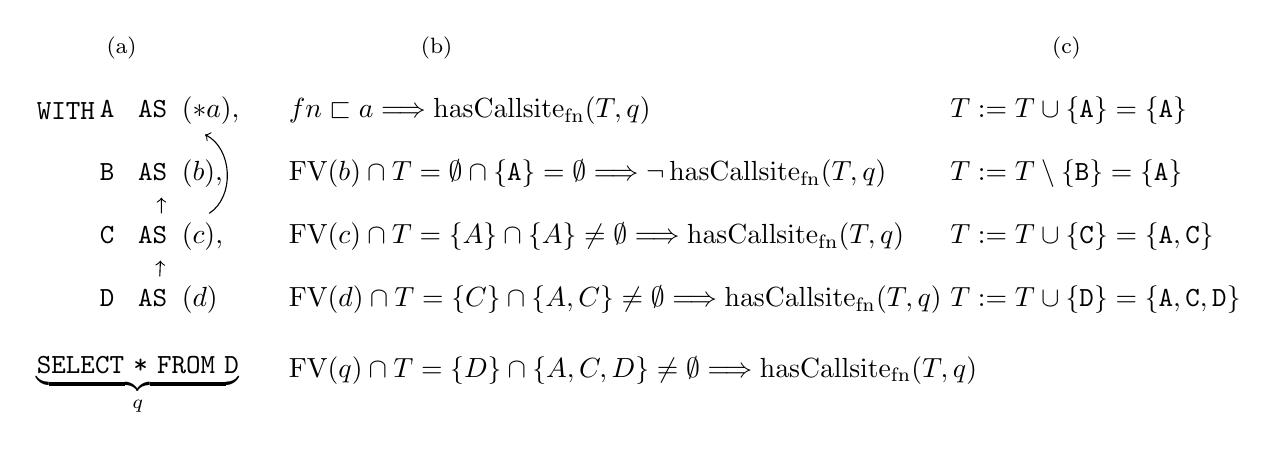
\begin{tikzpicture}[x=8mm, y=8mm]
    \node at (0.5, 1) {\footnotesize{(a)}};
    \node at (5.5, 1) {\footnotesize{(b)}};
    \node at (15.5, 1) {\footnotesize{(c)}};
    \node[anchor=west] at (-1, 0) {\WITH};
    \node[anchor=west] (A) at (0, 0)  {\texttt{A} \AS $(\ast a),$};
    \node[anchor=west] (B) at (0, -1) {\texttt{B} \AS $(b),$};
    \node[anchor=west] (C) at (0, -2) {\texttt{C} \AS $(c),$};
    \node[anchor=west] (D) at (0, -3) {\texttt{D} \AS $(d)$};
    \node[anchor=north west] (S) at (-1, -3.75) {$\underbrace{\SELECT~\texttt{*}~\FROM~\texttt{D}}_q$};
    \node[anchor=west] (Ar) at (3, 0)  {$fn \sqsubset a  \Longrightarrow  \hasCallsite(T, q)$};
    \node[anchor=west] (Br) at (3, -1) {$\FV(b) \cap T = \emptyset \cap \{\texttt{A}\} = \emptyset  \Longrightarrow  \neg \hasCallsite(T, q)$};
    \node[anchor=west] (Cr) at (3, -2) {$\FV(c) \cap T = \{A\} \cap \{A\} \neq \emptyset  \Longrightarrow  \hasCallsite(T, q)$};
    \node[anchor=west] (Dr) at (3, -3) {$\FV(d) \cap T = \{C\} \cap \{A, C\} \neq \emptyset  \Longrightarrow  \hasCallsite(T, q)$};
    \node[anchor=north west] (Dr) at (3, -3.75) {$\FV(q) \cap T = \{D\} \cap \{A, C, D\} \neq \emptyset  \Longrightarrow  \hasCallsite(T, q)$};
    \node[anchor=west] (Ar) at (13.5, 0) {$T := T \cup \{\texttt{A}\} = \{\texttt{A}\}$};
    \node[anchor=west] (Br) at (13.5, -1) {$T := T \setminus \{\texttt{B}\} = \{\texttt{A}\}$};
    \node[anchor=west] (Cr) at (13.5, -2) {$T := T \cup \{\texttt{C}\} = \{\texttt{A}, \texttt{C}\}$};
    \node[anchor=west] (Dr) at (13.5, -3) {$T := T \cup \{\texttt{D}\}= \{\texttt{A}, \texttt{C}, \texttt{D}\}$};
    \draw[->, bend right=60] (C) to (A);
    \draw[->] (C) to (B);
    \draw[->] (D) to (C);
    \end{tikzpicture}
    \caption{a) $q$ has no direct callsite, but reference \texttt{D} that contains a reference to \texttt{A} via \texttt{C}. \texttt{A} contains a direct callsite. b) A fragment $e$ is considered recursive if it contains a direct callsite ($fn \sqsubset$ e) or uses a recursive table-variable. c) If $\hasCallsite$ yields true for a CTE-body, its alias is added to the set of recursive table-variables $T$. Otherwise, the alias is removed to take into account shadowing.}
    \label{fig:my_label}
\end{figure}


\subsection{Tracking CTE-dependencies}\label{tracking_cte_dependencies}

\begin{align*}
    \refs(t) &:= \sigma_a(C[FV(T, t)]) \cup (\cup_{r \in \sigma_r(C[FV(T, t)])\}} r)
\end{align*}

\begin{figure}[h]
    \centering
    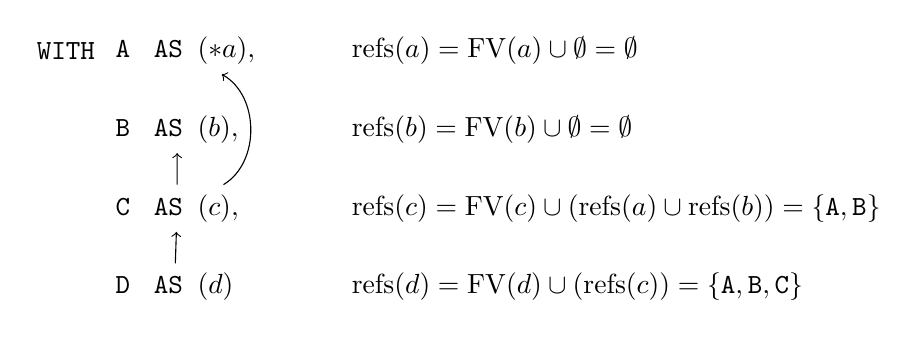
\begin{tikzpicture}[x=10mm, y=10mm]
    \node[anchor=west] at (-1, 0) {\WITH};
    \node[anchor=west] (A) at (0, 0)  {\texttt{A} \AS $(\ast a),$};
    \node[anchor=west] (B) at (0, -1) {\texttt{B} \AS $(b),$};
    \node[anchor=west] (C) at (0, -2) {\texttt{C} \AS $(c),$};
    \node[anchor=west] (D) at (0, -3) {\texttt{D} \AS $(d)$};
    \node[anchor=west] (Ar) at (3, 0)  {$\refs(a) = \FV(a) \cup \emptyset = \emptyset$};
    \node[anchor=west] (Br) at (3, -1) {$\refs(b) = \FV(b) \cup \emptyset = \emptyset$};
    \node[anchor=west] (Cr) at (3, -2) {$\refs(c) = \FV(c) \cup (\refs(a) \cup \refs(b)) = \{\texttt{A}, \texttt{B}\}$};
    \node[anchor=west] (Dr) at (3, -3) {$\refs(d) = \FV(d) \cup (\refs(c)) = \{\texttt{A}, \texttt{B}, \texttt{C}\}$};
    \draw[->, bend right=60] (C) to (A);
    \draw[->] (C) to (B);
    \draw[->] (D) to (C);
    \end{tikzpicture}
    \caption{References are tracked incrementally by collecting free table-variables (ie. direct CTE references) along with the references of those free table-variables.}
    \label{fig:my_label}
\end{figure}


\begin{wrapfigure}{r}{0.5\textwidth}
    \begin{minted}[autogobble]{sql}
        WITH T AS (SELECT 1)
        SELECT *
        FROM (
          WITH T AS (SELECT 2)
          SELECT * FROM T
        ) T
    \end{minted}
    \caption{The outer CTE \texttt{T} is shadowed by an inner CTE. The result of the query is \texttt{2}.}
    \label{lst:indirect_callsite_ref}
\end{wrapfigure}
When tracking table-variables within a scope, we may encounter the effect of \textit{shadowing}. A newly declared variable overrides an existing one of the outer scope. This is an important effect we need to take care of when tracking recursive table variables. \mintinline{psql}{SELECT (SELECT T.v FROM (SELECT f(n-1)) AS T(v)) FROM (SELECT 1) AS T(v)}. The row-reference \texttt{T(v)} is first declared (nonrecursivly) by the outer query and the overridden by the inner query inside \SELECT with a new, recursive definition.


\begin{figure}[h]
    \centering
    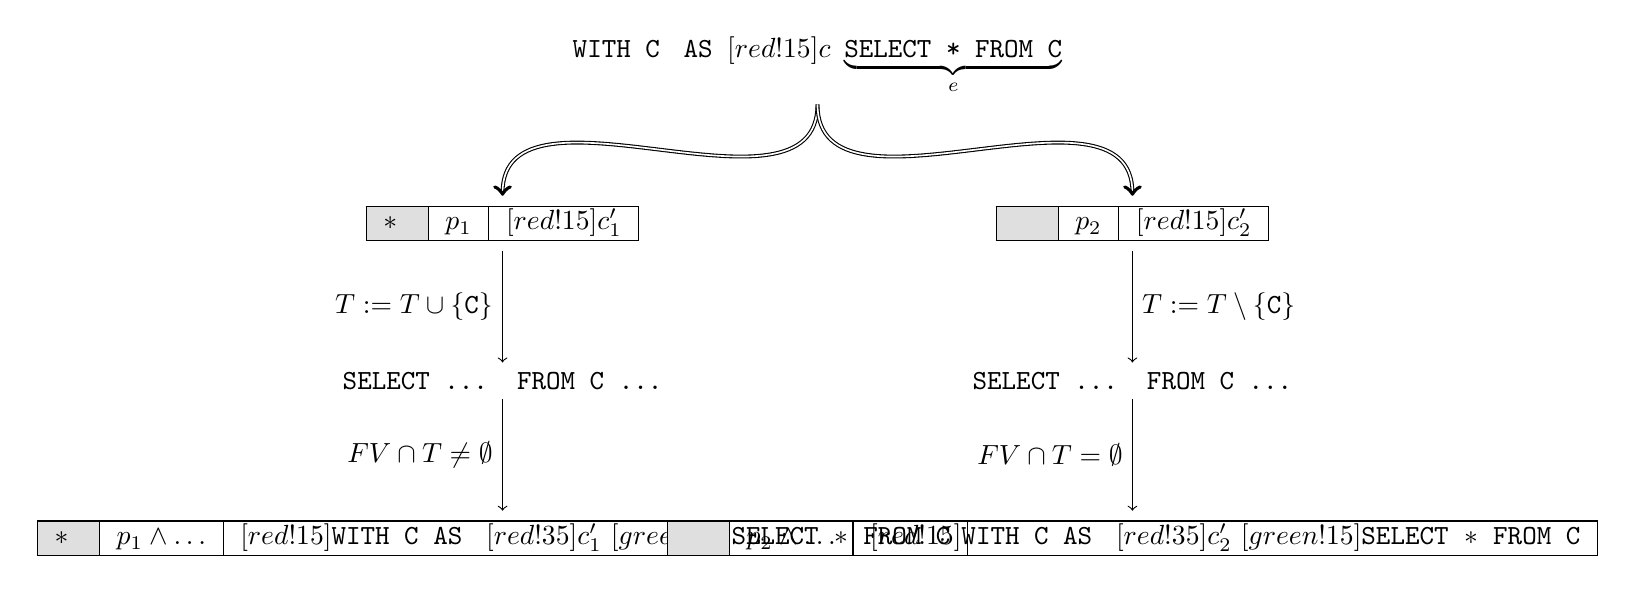
\begin{tikzpicture}
    \node (cte) at (4, 1) {\texttt{WITH C} \AS $\highlight[red!15]{c}~ \underbrace{\texttt{SELECT * FROM C}}_e$};
    \node (cte1) at (0, -1) {
        \begin{tabular}{|p{1em}|r|c|}\hline
        \cellcolor{gray!25} $\ast$ & $p_1$ & $\highlight[red!15]{c'_1}$\\\hline
        \end{tabular}
    };
    \node (cte2) at (8, -1) {
        \begin{tabular}{|p{1em}|r|c|}\hline
        \cellcolor{gray!25} & $p_2$ & $\highlight[red!15]{c'_2}$\\\hline
        \end{tabular}
    };
    \node (select1) at (0, -3) {\texttt{SELECT ... FROM C ...}};
    \node (select2) at (8, -3) {\texttt{SELECT ... FROM C ...}};
    \node (r1) at (0, -5) {
        \begin{tabular}{|p{1em}|r|c|}\hline
        \cellcolor{gray!25} $\ast$ & $p_1 \land \hdots$ & $\highlight[red!15]{\texttt{WITH C AS } ~\highlight[red!35]{c'_1}}~\highlight[green!15]{\SELECT~*~\texttt{FROM C}}$\\\hline
        \end{tabular}
    };
    \node (r2) at (8, -5) {
        \begin{tabular}{|p{1em}|r|c|}\hline
        \cellcolor{gray!25} & $p_2 \land \hdots$ & $\highlight[red!15]{\texttt{WITH C AS } ~\highlight[red!35]{c'_2}}~\highlight[green!15]{\SELECT~*~\texttt{FROM C}}$\\\hline
        \end{tabular}
    };
    \draw[->, double, out=270, in=90] (cte) to (cte1.north);
    \draw[->, double, out=270, in=90] (cte) to (cte2.north);
    \draw[->] (cte1.south) --node[left] {$T := T \cup \{\texttt{C}\}$} (select1);
    \draw[->] (cte2.south) --node[right]{$T := T \setminus \{\texttt{C}\}$} (select2);
    \draw[->] (select1) --node[left] {$FV \cap T \neq \emptyset$} (r1);
    \draw[->] (select2) --node[left] {$FV \cap T = \emptyset$} (r2);
    \end{tikzpicture}
    \caption{}
    \label{fig:my_label}
\end{figure}

The major difference to the \REXPR-rule is that new table-variables are introduces by \FROM, possibly shadowing out outer recursive tables. To reflect this behaviour, we remove all entries from $T$ that are shadowed by the newly introduced table-variables and add those of the newly introduces tables, that are recursive.
But there is one more thing we have to consider: By the fact that the \FROM-part introduces at least one recursive table-variable that is most likely used within \SELECT or \WHERE of the query, we would find out that those parts of the query are also recursive (since they referece a recursive table), violating the overall constraints and rendering the \FROM-rule useless. To avoid this, it is crucial to remove the shadowed table-variables from $T$ but not adding the newly recursive table-variables when checking if \SELECT and \WHERE have a callsite. This way, we allow only referencing only recursive tables introduces by this very query, but forbid any other recursive references.
\sqlcode{snippets/from_shadowing.sql}
\iffalse OLD
$$\quad(\textsc{from})\inferrule{
    \exists i \in \{1, ..., n\}: T \vdash \hasCallsite(e_{f_i}) \\
    T[a_1 \mapsto \bot, ..., a_n \mapsto \bot] \vdash \neg \hasCallsite(e_s) \land \neg \hasCallsite(e_w) \\
    \forall i \in \{1, ..., n\}: T, \varnothing \vdash (\TRUE, t_i) \rightarrow (B_i, R_i)
}{
    T, \varnothing \vdash (p, \SELECT e_s \FROM t_1 \AS a_1 \otimes ... \otimes  t_n \AS a_n \WHERE e_w) \rightarrow \\\\
    {\begin{tabular}[b]{LLLL}
    (~~&\{&(&\SELECT p ~\AND~ p_1 ~\AND~ \cdots ~\AND~ p_n, \\
          &&&\SELECT e_s \FROM t'_1 \AS a_1 \otimes ... \otimes  t'_n \AS a_n \WHERE e_w ~~)\\
      && | &~((p_1, t'_1), ..., (p_n, t'_n)) \in \times_{\{i|1\leq i \leq n\}} B_i\}, \\
    &\{&(&\SELECT p_1 ~\AND~ \cdots ~\AND~ p_n, \\
       &&&\SELECT e_s \FROM t'_1 \AS a_1 \otimes ... \otimes  t'_n \AS a_n \WHERE e_w ~~)\\
       &&| &~ ((p_1, t'_1), ..., (p_n, t'_n)) \in \times_{\{i|1\leq i \leq n\}} (B_i \cup R_i), \exists t' \in \{t'_1, ..., t'_n\} : \hasCallsite(t')\})\\
    \end{tabular}}
}$$
\fi
$$\quad(\textsc{from})\inferrule{
    \exists i \in \{1, ..., n\}: \hasCallsite(T, e_{f_i}) \\
    \neg \hasCallsite(T, e_s)\\
    \neg \hasCallsite(T, e_w) \\\\
    \forall i \in \{1, ..., n\}: T, \varnothing \vdash (\TRUE, t_i) \rightarrow (B_i, R_i)
}{
    T, \varnothing \vdash (p, \SELECT~ e_s ~\FROM~ t_1 \AS a_1 \otimes ... \otimes  t_n \AS a_n ~\WHERE~ e_w) \rightarrow \\\\
    {\begin{tabular}[b]{LLLL}
    (~~&\{&(&\SELECT~ p ~\AND~ p_1 ~\AND~ \cdots ~\AND~ p_n, \\
          &&&\SELECT~ e_s ~\FROM~ t'_1 \AS a_1 \otimes ... \otimes  t'_n \AS a_n ~\WHERE~ e_w ~~)\\
      && | &~((p_1, t'_1), ..., (p_n, t'_n)) \in \times_{\{i|1\leq i \leq n\}} B_i\}, \\[6pt]
    &\{&(&\SELECT~ p_1 ~\AND~ \cdots ~\AND~ p_n, \\
       &&&\SELECT~ e_s ~\FROM~ t'_1 \AS a_1 \otimes ... \otimes  t'_n \AS a_n ~\WHERE~ e_w ~~)\\
       &&| &~ ((p_1, t'_1), ..., (p_n, t'_n)) \in \times_{\{i|1\leq i \leq n\}} (B_i \cup R_i), \exists t' \in \{t'_1, ..., t'_n\} : \hasCallsite(t')\}\\
    )\\
    \end{tabular}}
}$$

\subsection{\RCTE-rule: Collecting and analyzing CTE-Scenarios}
CTE-Scenarios are computed and dependencies for the scenarios are collected.
$$\quad(\textsc{cte})\inferrule{
    \hasCallsite(T, \WITH a_1 \AS t_1, ..., a_n \AS t_n~q)\\
    T, \varnothing \vdash (p, t_1) \rightarrow (B, R) \\
    ((B \times \{\bot\}) \cup (R \times \{\top\})) = \{(p'_{t_1}, t'_1, r_{i_1}), ..., (p'_{t_k}, t'_k, r_k)\} = X\\
    \forall (p'_t, t', r_i) \in X: T[a_1 \mapsto r_i], C[a_1: (t', p'_t, FV^+(t')] \vdash (p, \WITH a_2 \AS t_2, ..., a_n \AS t_n~q) \rightarrow (B_i, R_i)
}{
    T, C \vdash (p, \WITH a_1 \AS t_1, ..., a_n \AS t_n~q) \rightarrow ((\cup_{1 \leq i \leq k} B_i), (\cup_{1 \leq j \leq k} R_j)\})
}$$

$$\quad(\textsc{cte})\inferrule{
    T \vdash \hasCallsite(\WITH~ a_1 \AS t_1, ..., a_n \AS t_n~q)\\
    T, \varnothing \vdash (p, t_1) \rightarrow (B, R) \\
    \forall (p'_t, t') \in B: T \setminus \{a_1\}, C[a_1: (t', p'_t, FV^+(t')] \vdash (p, \WITH~ a_2 \AS t_2, ..., a_n \AS t_n~q) \rightarrow (B_i, R_i) \\
    \forall (p'_t, t') \in R: T \cup \{a_1\}, C[a_1: (t', p'_t, FV^+(t')] \vdash (p, \WITH~ a_2 \AS t_2, ..., a_n \AS t_n~q) \rightarrow (B_j, R_j)
}{
    T, C \vdash (p, \WITH~ a_1 \AS t_1, ..., a_n \AS t_n~q) \rightarrow ((\cup_{1 \leq i \leq k} B_i) \cup (\cup_{1 \leq j \leq l} B_j), (\cup_{1 \leq j \leq k} R_j) \cup (\cup_{1 \leq j \leq l} R_j)\})
}$$

\subsection{\RWITH-rule: Attaching used CTEs only}
When all CTEs at a level are processed, the actual query is processed independently. The query contains none of the preceeding CTEs anymore, so that it is sufficient to analyze the current subtree together with the set $T$ of recursive CTEs in scope to decide whether a subtree is recursive.
$$\quad(\textsc{with})\inferrule{
    C \neq \varnothing\\
    T, \varnothing \vdash (p, q) \rightarrow (B, R)
}{
    T, C \vdash (p, \WITH q) \rightarrow \\\\
    {\begin{tabular}[b]{LLLL}
    (~~&\{&(&\WITH [a_i \AS t_i]^{(a_i, t_i) \in \sigma_{a, t}(q'_{ctePreds})}~\SELECT (\AND_{p_i \in \{p_q\} \cup \sigma_p(q'_{ctes})} p_i), \\
          &&&\WITH [a_i \AS t_i]^{(a_i, t_i) \in \sigma_{a, t}(q'_{ctes})}~~q'~\\
          &&| &~(p_q, q') \in B,~ q'_{ctes} = C[FV^+(q')],~ q'_{ctePreds} = C[\cup_{x_p \in \{p_q\} \cup \sigma_p(q'_{ctes})} FV^+(x_p)]\},\\
    &\{&(&\WITH [a_i \AS t_i]^{(a_i, t_i) \in \sigma_{a, t}(q'_{ctePreds})}~\SELECT (\AND_{p_i \in \{p_q\} \cup \sigma_p(q'_{ctes})} p_i), \\
    &&&\WITH [a_i \AS t_i]^{(a_i, t_i) \in \sigma_{a, t}(q'_{ctes})}~~q'~\\
    &&|&~(p_q, q') \in R,~ q'_{ctes} = C[FV^+(q')],~ q'_{ctePreds} = C[\cup_{x_p \in \{p_q\} \cup \sigma_p(q'_{ctes})} FV^+(x_p)])
    \end{tabular}}
}$$
\\



\section{Postprocessing of the scenarios}
\subsection{Extraction of callsite-arguments}
We need to extract the arguments of the callsites within a recursive case, eg: 
\begin{minted}{sql}
SELECT T.a + T.b + T.c FROM (SELECT f(n-1, 2), 3, 4 + f(5, 6) FROM T WHERE p) AS T(a, b, c)
\end{minted}
into a set of callsite-arguments with its arguments $\{(\SELECT n-1, \SELECT 2), (\SELECT 5, \SELECT 6)\}$. As we require the callsite-arguments to be uncorrelated, we do not have to deal with references to \FROM but only to CTEs, wich simplifies things greatly.

Remove sourrinding query if callsite is within \SELECT, because the value of the callsite-arguments must be invariant to the tables references in \FROM.
$$\quad(\textsc{select})\inferrule{
    \exists i \in \{1, ..., n\}: \text{containsCallsite}(s_i) \\
    \forall i \in \{1, ..., n\}: \varnothing \vdash s_i \rightarrow P_i
}{
    \varnothing \vdash \SELECT s_1, ..., s_n \FROM f \WHERE w \rightarrow \\\\
    \{(\SELECT e_1, ..., \SELECT e_k) | (e_1, ..., e_k) \in \cup_{i \in \{1, ..., n\}} P_i \}
}$$

Remove outer query if callsite is within FROM, because sourrounding query is irrelevant for evaluation of subqueries in FROM.
$$\quad(\textsc{from})\inferrule{
    \forall i_j \in \{i_1, ...., i_m\} \subseteq \{1, ..., n\}: \text{containsCallsite}(f_{i_j})\\
    \forall i_j \in \{i_1, ...., i_m\}: \varnothing \vdash f_{i_j} \rightarrow P_{i_j}
}{
    \varnothing \vdash \SELECT s \FROM a_1 \AS f_1 \otimes ... \otimes a_n \AS f_n \WHERE w \rightarrow \cup_{i \in \{1, ..., n\}} P_i
}$$

Evaluate CTEs seperately, keeping previous CTEs that are referenced, in the case that there are callsites inside CTEs. Saving also every CTE to the CTE-store if they are references form the actual query.
$$\quad(\textsc{cte})\inferrule{
    \varnothing \vdash t_1 \rightarrow P \\
    C[a_1 : (t_1, FV^+(C, t_1))] \vdash \WITH a_2 \AS t_2, ..., a_n \AS t_n ~q \rightarrow P_w
}{
    C \vdash \WITH a_1 \AS t_1, ..., a_n \AS t_n ~q \rightarrow \\\\
    \{(\WITH [a_i \AS t_i]_{(a_i, t_i) \in C[FV^+(e_1)]} ~e_1, ..., \WITH [a_i \AS t_i]_{(a_i, t_i) \in C[FV^+(e_m)]} ~e_m) | (e_1, ..., e_m) \in P\} \cup P_w
}$$


$$\quad(\textsc{with})\inferrule{
    \varnothing \vdash q \rightarrow P
}{
    C \vdash \WITH q \rightarrow \\\\
    \{(\WITH [a_i \AS t_i]_{(a_i, t_i) \in C[FV^+(e)]} ~e_1, ..., \WITH [a_i \AS t_i]_{(a_i, t_i) \in C[FV^+(e_m)]} ~e_m) | (e_1, ..., e_m) \in P\}
}$$

Remove surrounding expression for every branch that contains a callsite, collecting results of all arguments.
$$\quad(\textsc{expr})\inferrule{
    \exists i \in \{1, ...., n\}: \text{containsCallsite}(e_i)\\
    \forall i \in \{1, ...., n\}: \varnothing \vdash e_i \rightarrow P_i
}{
    \varnothing \vdash \text{expr}(e_1, e_2, ..., e_n) \rightarrow \cup_{i \in \{1, ...., n\}} P_i
}$$

Remove recursive call and collect args.
$$\quad(\textsc{call})\inferrule{
}{
    \varnothing \vdash fn_{rec}(e_1, e_2, ..., e_n) \rightarrow \{ (e_1, e_2, ..., e_n) \}
}$$

If subbranch contains no callsite, stop and return empty set.
$$\quad(\textsc{nocall})\inferrule{
\neg \text{containsCallsite}(e)
}{  
    \varnothing \vdash e \rightarrow \{\}
}$$

Callsites within aggregate-functions are forbidden by the restriction that there must be a static number of callsites. Looping through a table, evaluating a recursive call per row is not allowed.



\chapter{Translation Templates}

\section{Callstack discovery}

\begin{minted}{SQL}
SELECT callsite_id, evaluate_arg_1_with_params(params)
FROM predicate_of(scenario) AS p(v)
WHERE p.v
\end{minted}
\section{Callstack evaluation}

\section{Result selection}

\section{Handling nontermination}
Semantic equivalence requires the translation not only to return the same correct results, but also to behave equally in terms of (non)termination. Without special measures, our template will terminate returning a NULL value where the original function 
\subsection{Infinite callstack}
n-1, n-2, n-3, ... looping behaviour is same, callstack table grows forever

\subsection{Looping calls}
n-1, n-1, ... callstack table is finite => but no basecases are reached and evaluation will not start => force loop.

\subsection{Some basecases not reachable}
If only a part of the functions leads to looping calls, evaluation starts since there are basecases, but no final result can be outputted. Force loop.

\chapter{Optimizations}
\section{Handling unhashable types}
\subsection{Detection}
\subsection{Template optimization}

\section{Constant parameter removal}
\subsection{Detection}
\subsection{Template optimization}

\section{Tail Recursion}
\subsection{Detection}
If the result of a recursive call is not used for further computations, ie. the computation context can be disposed, the call is a tail call. If all recursive calls are tail calls, the function is tail recursive. We can utilize this property to skip the evaluation phase which computes the results of all expressions containing a recursive call. In the case of tail recursion the recursive expression equals the call itself, thus no evaluation is required. Usually, the evaluation-phase computes the result of a call with given input parameters by waiting for the results of the callsites and then compute the result of this function call by evaluating the recursive expression with the calls replaced by its results.

A tail recursive function do not need this evaluation phase, because there is no context that need to be evaluated. The context in question is the very call itself. Therefore it is possible to skip the evaluation phase and return directly the result of the last call.

We detect tail recursive calls by analyzing the structure of the recursive cases returned by the static analysis. The only possible strucutre of a tail recursive call is the following
\begin{minted}{SQL}
SELECT (SELECT (SELECT f(..)))
\end{minted}
A complete Example:
\sqlcode{snippets/udf_gcd.sql}

Any computations like \texttt{1+(SELECT f(n))} would create a context around the call that need to be evaluated. The same for \FROM, even if the callsite-arguments contain no table-references, we are required to loop through the rows and create the output table.

If a function is a tail call but its argument references a CTE and therefore the query is prefixed by an \WITH-block, it is still tail recursive, because the reference to any CTE is within the callsite arguments that are removed alltogether with the call during evaluation. So, during evaluation time, the CTEs are not used and thus could be removed, and the expression is tail recursive.
\subsection{Template optimization}

\section{Single Recursion}
\subsection{Detection}
\subsection{Template optimization}
Simple: only one callsite per 
Only one callsite => no need to wait for all callsites of a recursive call
no need to collect all callsites of a given recursive call
union all -> union...wieso?
\newpage

%%
\chapter{Evaluation and discussion}\label{results_discussion}
\section{Advantages} Moimization, memory limitation, query planner
\section{Original vs. Translation}
\subsection{Number of recursive cases}
\subsection{Number of basecases}
\subsection{Number of parameters}
\subsection{Branching factor}

\section{Optimizations}
\subsection{Linear Recursion}
\subsection{Tail Recursive}
\subsection{Constant Parameters}

\section{Bottlenecks}
\newpage

%%

\subsection{Properties of the translation}
Equivalence for mathematical functions is intuitively defined as $f: S \mapsto T, g: U \mapsto V, \forall x \in S: f(x) = g(x)$ with $S = U, T = V$. If the domain, ie. the function signature, matches and the results are equal for every input, the functions are considered to be equivalent. We have to extend this definition a little to bear the newly introduced aspects of real (database-)world procedures.

The signatures of a PostgreSQL-UDF does contain many different keywords reflecting properties of the function to give hints to the database-system how to UDF is callable or what kind of optimizations are applicable. Therefore, we require the translation not only to match the function signature (say: $gcd(int, int) : int$), but also the complete CREATE FUNCTION-block surrounding the actual function body. If a function is marked eg. as IMMUTABLE, the translation preserves this property. The only exception are UDFs that are marked PARALLEL SAFE, that is changed to PARALLEL RESTRICTED since the translation uses non-parallel safe operations like CTE-Scans (15.4. Parallel Safety).

In general, we cannot assume that UDFs are total, ie. that they terminate for all possible inputs from the input space. Assume a function that only terminates for positive inputs or may throw a division-by-zero error. This behaviour must be preserved by the translation, otherwise it would be not be clear if an error is actual a bug in the original function or introduced by the translation.

RETURNS NULL ON NULL INPUT/STRICT\\
VARIADIC (argument list)\\
DEFAULTs\\
argmodes?\\
positional vs named notation: breaks calls!





\section{Constraints of our approach}
Our approach can optimize a wide range of recursive UDFs, but there exist cases where a translation would not be beneficial or is not possible with my current implementation. I will characterize the set of translateable UDFs by formulating a number of constraints that must hold for a given query. Otherwise, the translation will fail or lead to an incorrect translation.
 
\subsection{No dependant callsites}
Our evaluation-strategy evaluates all callsites of an recursive expression independently and returns a result eventually only if all contained callsites have returned a result. For this reason, dependant callsites like $f(f(x))$ are not possible. Even more important is this constraint for \CASE-Statements. Imagine the following body of a recursive UDF \texttt{f}:
% TODO: Find more meaningful example
\begin{minted}{postgresql} 
SELECT CASE
  WHEN n      = 0 THEN 0
  WHEN f(n-1) = 0 THEN 1
  WHEN f(n-2) = 1 THEN 2
  ELSE 0
END;
\end{minted}
Here, the execution of the second \CASE-branch depends on the execution of the callsite in the first branch. After statically analysis, this block would result in one big recursive case with two callsites. The evaluation-strategy would execute both calls, leading to a behaviour possibly differing greatly from the original, eg. calling \texttt{f(n-2)} with invalid parameters leading to an infinite loop \texttt{(f(0), f(1)), (f(-1), f(-2), (f(-2), f(-3)), ...)}

\subsection{Explicit basecases required}
It is possible to write recursive functions that does not posses a basecase according to our static analysis, but do terminate and thus posses another way of terminating. Trivially, this can be achieved by using other conditionals as \CASE for case distinction like \texttt{GREATEST}, \texttt{LEAST}, \texttt{NULLIF} or \texttt{COALESCE}. Those functions can be viewed as syntactic sugar for \CASE since all of them can be formulated with \CASE only, see \ref{sql:cond_norm}. This could be done easilly in a normalizing preprocessing step.

But there exist more ways of formulating basecases which are harder do detect, like in the following example:
\sqlcode{snippets/no_basecases.sql}
Here, the basecase occurs when the table containing the recursive call is empty and therefore no recursive call happens. Examples like this show, that there is a variety of possibilities to write recursive functions without using an explicit \CASE. Translations for many of them may exist, but we focus in the following on recursive queries with explicit case-distinctions utilizing \CASE-expressions.

\subsection{Predicates and callsite-arguments may only reference CTEs and schema tables}
One challenge is slicing the function, the other is evaluating the arguments idependently from the surrounding query. While the first is mostly solved by my thesis, the latter is worth further examination to lift the constraints on callsite-arguments.

...

We require that predicates within a \texttt{CASE}-statement contain no references to row-varaibles like \texttt{T.v} that were introduced by an outer \FROM. This does not mean that no tables can be accessed. It is indeed possible to access tables, but these have to origin from an CTE, not a \FROM. This assumption is necessary to savely factor out the predicate which gets evaluated repeatably in the original implementation. This constraint can also be lifted if a table-compatible template is used for translation. The idea of the table-template is to replace all row variables by our own variables, alongside with the callsite-results. That way we have 
\sqlcode{snippets/predicates_must_be_selfcontained.sql}

The same goes for arguments of callsites.

\begin{listing}[ht]
\sqlcode{snippets/predicate_with_outside_references.sql}
\caption{Example of a (forbidden) predicate that has references to outside tables and thus returns a table of predicates.}
\label{lst:from_nonselfcontained}
\end{listing}
\newpage

%%
\input{4_Forschungsstand}
\newpage

%%
\chapter{Conclusion and future work} \label{conclusion}
Analyzing the callstack to limit rows needed to carry around
Remove calls from the callstack when all dependant calls are evauated

\section{\texttt{STRICT} functions}
Functions tagged as \texttt{STRICT} are functions that return \texttt{NULL} straight away if they any of their arguments is \texttt{NULL}. The actual function is not evaluated in this case. In this case no call with a \textit{NULL} argument will lead to subsequent callsites, so that all recursive scenarios have non-\texttt{NULL} arguments. Calls with a \texttt{NULL}-argument are therefore only required to consider when collecting basecases. During evaluation all arguments are not nullable and \texttt{x IS NOT DISTINCT FROM y} can be simplified to \textit{x = y}. This may yield to a large performance gain as the implicit \texttt{x = y OR (x IS NULL AND y IS NULL)} is removed wich degrades join-performance.

\section{Closures of SQL-fragments containing row-variables}
\section{Tabular return types}
\section{Evaluation of predicate-parts in own CTE}
\section{Parallel execution of in dependant callstack-subtrees}
\section{Iterative recursive calls to limit size of evaluation-table}
\section{Indices}
\section{Translation from and to other languages}

Single callsite => no calsite id required

%%%%%%%%%%%%%%%%%%%%%%%%%
% Was war das Ziel?
% Was habe ich getan?
% Was wurde erreicht?
% Was lernen wir daraus?
% "Woran könnte man weiter forschen?"
%%%%%%%%%%%%%%%%%%%%%%%%%
\section*{Acknowledgements}
Thanks to Chris, Denis, Grust, proofreader, ...
\newpage

%%
\cleardoublepage
\renewcommand{\thesection}{\Alph{section}}%
%\appendix 
%\addcontentsline{toc}{chapter}{Anhang} 

%%%%%%%%%%%%%%%%%%%%%%%%
%%%%%%%%%%%%%%%%%%%%%%%%
%%%%%%%%%%%%%%%%%%%%%%%%
\chapter[Appendix]{Appendix}
\phantomsection
\section{Example translations}
\subsection{\texttt{fib}}
\begin{figure}\footnotesize
    \centering
    \sqlcode{snippets/fib_callstack.sql}
    \caption{\texttt{callstack}-CTE as standalone query. Note that the UDF argument \texttt{\$1} is replaced with a SQL-variable \texttt{:n}}
    \label{fib:callstack_cte_complete}
\end{figure}
\section{Conditional normalization}
\sqlcode{snippets/conditional_normalization.sql}\label{sql:cond_norm}
%%%%%%%%%%%%%%%%%%%%%%%%


%%%%%%%%%%%%%%%%%%%%%%%%%%%%%%%%%%%%%%%%%%%%%%%%%%%%%%%%%%%%%%%%%%%%%%%%%%%%%
%%% Bibliographie
%%%%%%%%%%%%%%%%%%%%%%%%%%%%%%%%%%%%%%%%%%%%%%%%%%%%%%%%%%%%%%%%%%%%%%%%%%%%%

\addcontentsline{toc}{chapter}{Bibliography}
\bibliographystyle{alpha}
\bibliography{mylit}
%% Obige Anweisung legt fest, dass BibTeX-Datei `mylit.bib' verwendet
%% wird. Hier koennen mehrere Dateinamen mit Kommata getrennt aufgelistet
%% werden.

\cleardoublepage

%%%%%%%%%%%%%%%%%%%%%%%%%%%%%%%%%%%%%%%%%%%%%%%%%%%%%%%%%%%%%%%%%%%%%%%%%%%%%
%%% Erklaerung
%%%%%%%%%%%%%%%%%%%%%%%%%%%%%%%%%%%%%%%%%%%%%%%%%%%%%%%%%%%%%%%%%%%%%%%%%%%%%
\thispagestyle{empty}
\section*{Selbst\"andigkeitserkl\"arung}

Hiermit versichere ich, dass ich die vorliegende Masterarbeit 
selbst\"andig und nur mit den angegebenen Hilfsmitteln angefertigt habe und dass alle Stellen, die dem Wortlaut oder dem 
Sinne nach anderen Werken entnommen sind, durch Angaben von Quellen als 
Entlehnung kenntlich gemacht worden sind. 
Diese Masterarbeit wurde in gleicher oder \"ahnlicher Form in keinem anderen 
Studiengang als Pr\"ufungsleistung vorgelegt. 

\vskip 3cm

Ort, Datum	\hfill Unterschrift \hfill 

\end{document}